\documentclass{report}
\usepackage{subfig}
\usepackage{graphicx}
\usepackage{float}
\usepackage[margin=1in]{geometry}
\usepackage{indentfirst}
\graphicspath{ {./images/} }
\DeclareGraphicsExtensions{.pdf}

\begin{document}

\title{\textbf{Project Watt} \\ LCOM Final Report \\ Turma 6 - Grupo 7}
\author{Eduardo da Costa Correia\\
\texttt{up201806433}
\and
Tiago Duarte Silva\\
\texttt{up201806516}}   
\maketitle

\tableofcontents

\chapter{Instruções de Utilização} 

\section{Menu Principal}

Ao iniciar o programa, é apresentada o menu principal, onde o jogador pode selecionar um dos dois modos de jogos possíveis a iniciar, cada um com a opção de se jogar ou não com outro jogador (se for para jogar em modo \textbf{Co-Op}, um computador deve selecionar Co-op P1 e o outro Co-op P2).

Para sair do jogo, o utilizador deve pressionar a tecla \textbf{\textit{Esc}} duas vezes, o mesmo para voltar ao menu principal a partir de um dos modos de jogo.

\begin{figure}[H]
	\centering
	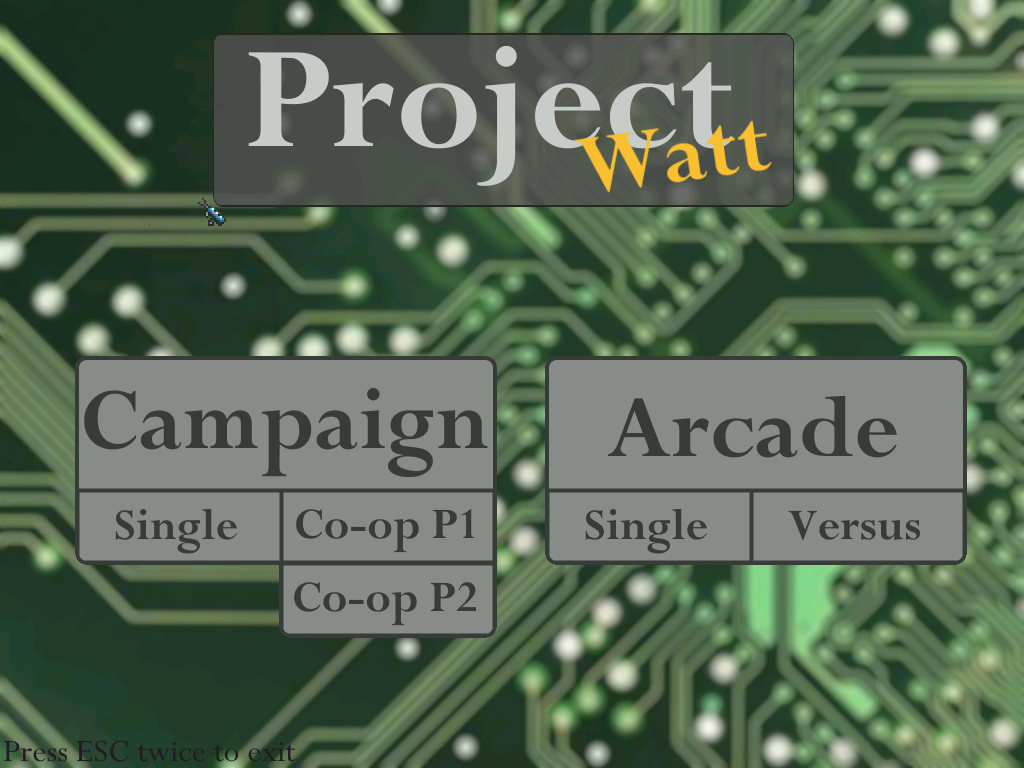
\includegraphics[width=0.9\textwidth]{main_menu}
	\caption{Menu principal}
\end{figure}

\pagebreak

\section{Campaign}

Este é o modo de jogo "principal", que se trata de um \textit{platformer} em que um jogador controla a personagem \textit{Watt} (Figura \ref{fig:watt}), uma faísca que ficou "presa" num curto-circuito e que para sair terá de fazer "ligação à terra" (Figura \ref{fig:exit}), ou seja, neste caso, a personagem tem de alcançar o \textbf{canto superior direito do mapa} (Figura \ref{fig:level}\footnotemark). Para isso tem de ultrapassar diversos obstáculos tais como os \textbf{espinhos} e \textbf{lasers} (se tocar num destes a faísca dissipa-se e volta ao início).

Para além disso, é possível controlar certos aspetos da jogabilidade, como a \textbf{altura do salto} da personagem e a sua \textbf{velocidade} (através dos \textit{sliders} azul e laranja respetivamente). 

Existem ainda dois \textbf{powerups} que após obtidos, desbloqueiam o controlo de funcionalidades adicionais, requeridas para acabar o nível. Estes são o powerup dos \textbf{lasers} (\textbf{canto superior esquerdo} - Figura 1.3) que permitem controlar qual dos lasers está \textbf{inativo} (vermelho, azul ou roxo - através dos botões com a cor correspondente) e alterar o sentido da gravidade da personagem (ou seja, a personagem passa a ser puxada para cima em vez de para baixo como seria normalmente). 

Todos estes aspetos são controlados pelo \textbf{segundo jogador}, se estiver a jogar em co-op através de uma \textbf{\textit{switchboard}} (Figura \ref{fig:switchboard}). Esta \textbf{\textit{switchboard}} possui ainda um \textbf{\textit{mini-jogo}} que consiste em destruir \textbf{\textit{balões}} que aparecem (clicando neles) antes que estes atinjam o \textbf{topo do ecrã}, caso contrário, tal gerará \textbf{\textit{interferência}} (o ecrã fica com \textit{ruído} para tornar a experiência mais desafiante e fazer com que quem controle a personagem 2 tenha de estar mais ativo).

\begin{figure}[H]
	\centering
	
\includegraphics{watt}
	\caption{Personagem 1 - Watt}
	\label{fig:watt}
\end{figure}

\begin{figure}[H]
	\centering
	
\includegraphics[width=0.08\textwidth]{exit_icon}
	\caption{Saída}
	\label{fig:exit}
\end{figure}

\begin{figure}[H]
    \centering
    \subfloat[Laser]{{
\includegraphics{laser_icon} }}%
    \qquad
    \subfloat[Anti-gravidade]{{
\includegraphics{anti_gravity_icon} }}
    \caption{Powerups}
    \label{fig:powerups}
\end{figure}

\footnotetext{As figuras apresentadas para ilustrar o nível da personagem 1 do modo campaign são do modo singleplayer, portanto incluem botões e \textit{sliders} no canto superior esquerdo que não estão presentes no modo \textit{co-op}}

\pagebreak

\begin{figure}[H]
	\centering
	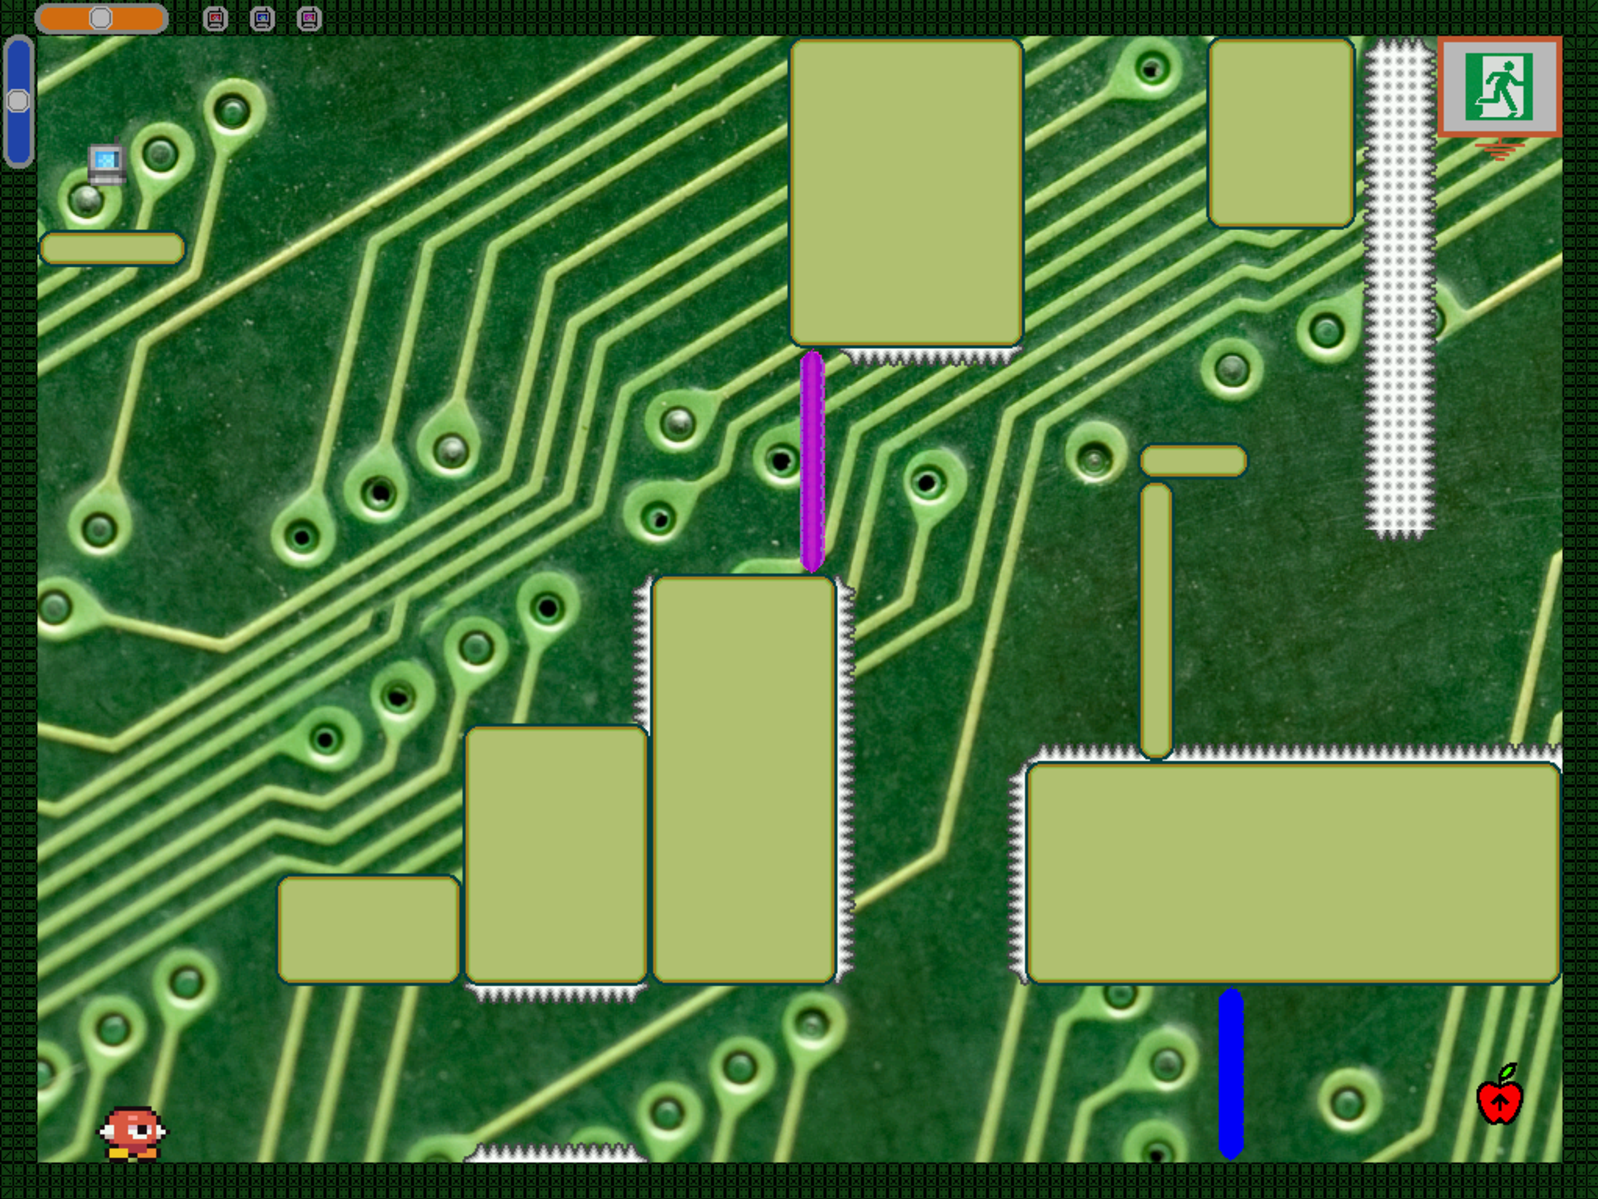
\includegraphics[width=0.8\textwidth]{campaign_singleplayer}
	\caption{Campaign - Nível (Personagem 1)}
	\label{fig:level}
\end{figure}

\begin{figure}[H]
	\centering
	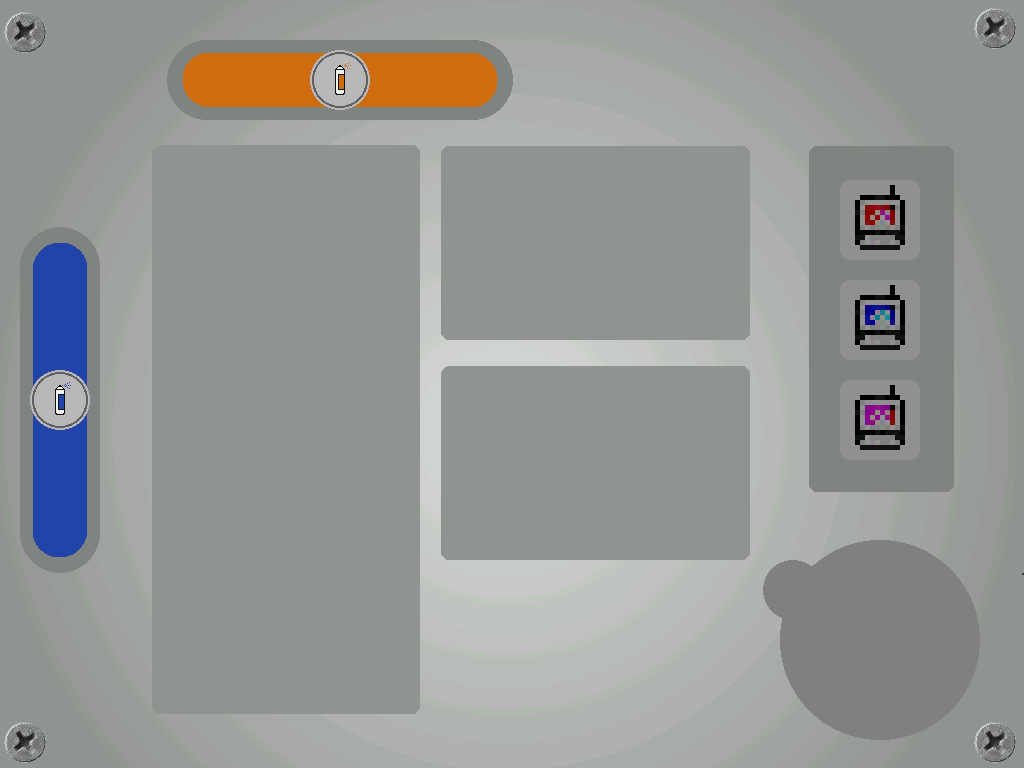
\includegraphics[width=0.8\textwidth]{campaign_switchboard}
	\caption{Campaign - Switchboard (Personagem 2)}
	\label{fig:switchboard}
\end{figure}

\pagebreak

\subsection{Victory Screen}

Quando o jogador conclui o modo \textbf{\textit{Campaign}}, é exibido um ecrã a parabenizá-lo e a informá-lo do \textbf{tempo que demorou}, em segundos, a fazê-lo.
Para sair deste ecrã e regressar ao menu principal o utilizador deve pressionar \textbf{\textit{Esc}} duas vezes.

\begin{figure}[H]
	\centering
	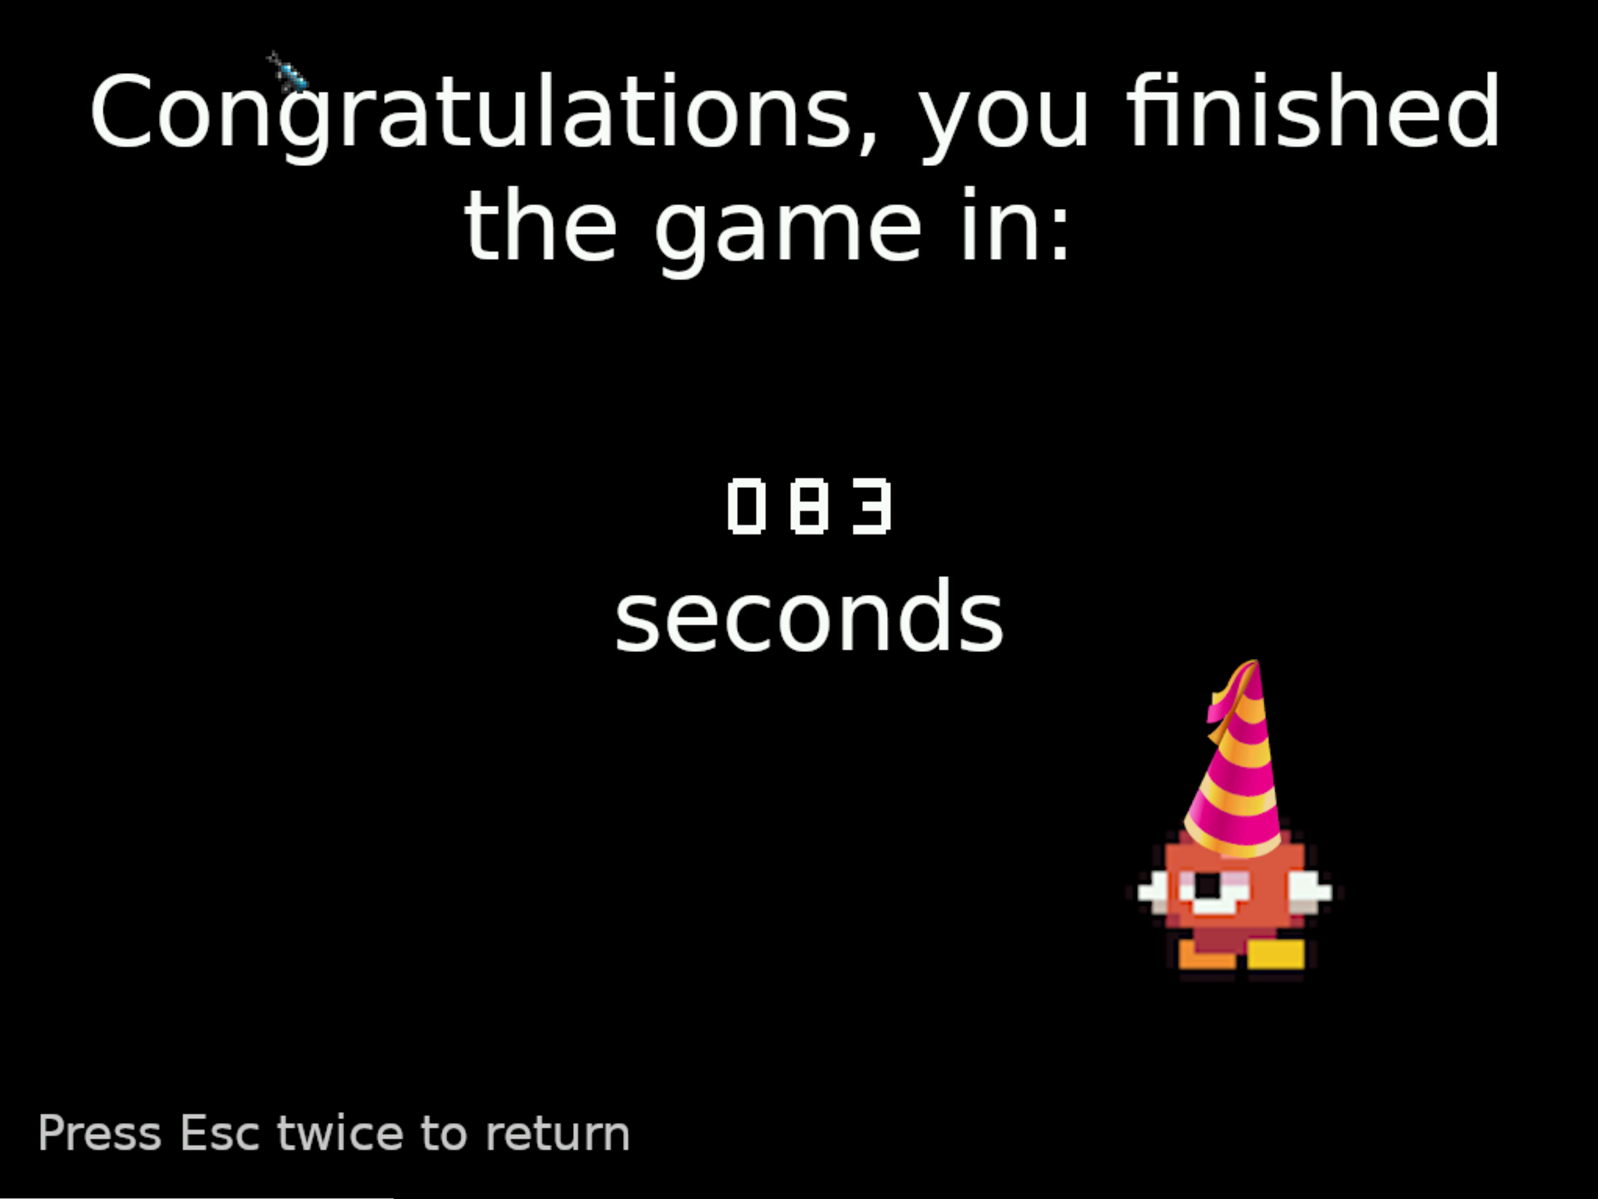
\includegraphics[width=0.8\textwidth]{win_screen}
	\caption{Campaign - Victory Screen}
\end{figure}

\pagebreak

\section{Arcade}

\textbf{\textit{Arcade}} é um modo de jogo alternativo, baseado na mecânica de \textbf{anti-gravidade} do outro modo de jogo. Neste o jogador terá de se desviar de \textbf{lasers} que vêm na sua direção (passando por entre estes) tentanto aguentar o máximo de tempo possível sem tocar neles e perder. Por cada par de \textbf{lasers} que o jogador passa o seu \textbf{\textit{score}} (\textbf{canto superior direito} - Figura \ref{fig:arcade_singleplayer}) aumenta por um ponto. O \textbf{\textit{score}} superior, a \textbf{branco}, representa a sua pontuação atual (que é reposta de cada vez que este toca num \textbf{laser}), já o \textbf{\textit{score}} inferior, a \textbf{cinzento}, representa a maior pontuação (\textbf{\textit{highscore}}) do jogador que ele conseguiu obter durante a partida.

Possui também um modo \textbf{\textit{versus}} (Figura \ref{fig:arcade_versus}), em que dois utilizadores jogam simultaneamente para ver quem obtém a maior pontuação durante um tempo limite (de 45 segundos, após o qual aparece um ecrã a informar de quem foi a vitória e a pontuação respetiva de cada jogador - Figura \ref{fig:arcade_you_win}). Para distinguir entre os dois jogadores, um deles é apresentado com uma cor \textbf{azulada}, tal como o seu \textbf{\textit{score}} e o outro a vermelho (Figura \ref{fig:arcade_versus}).

\begin{figure}[H]
	\centering
	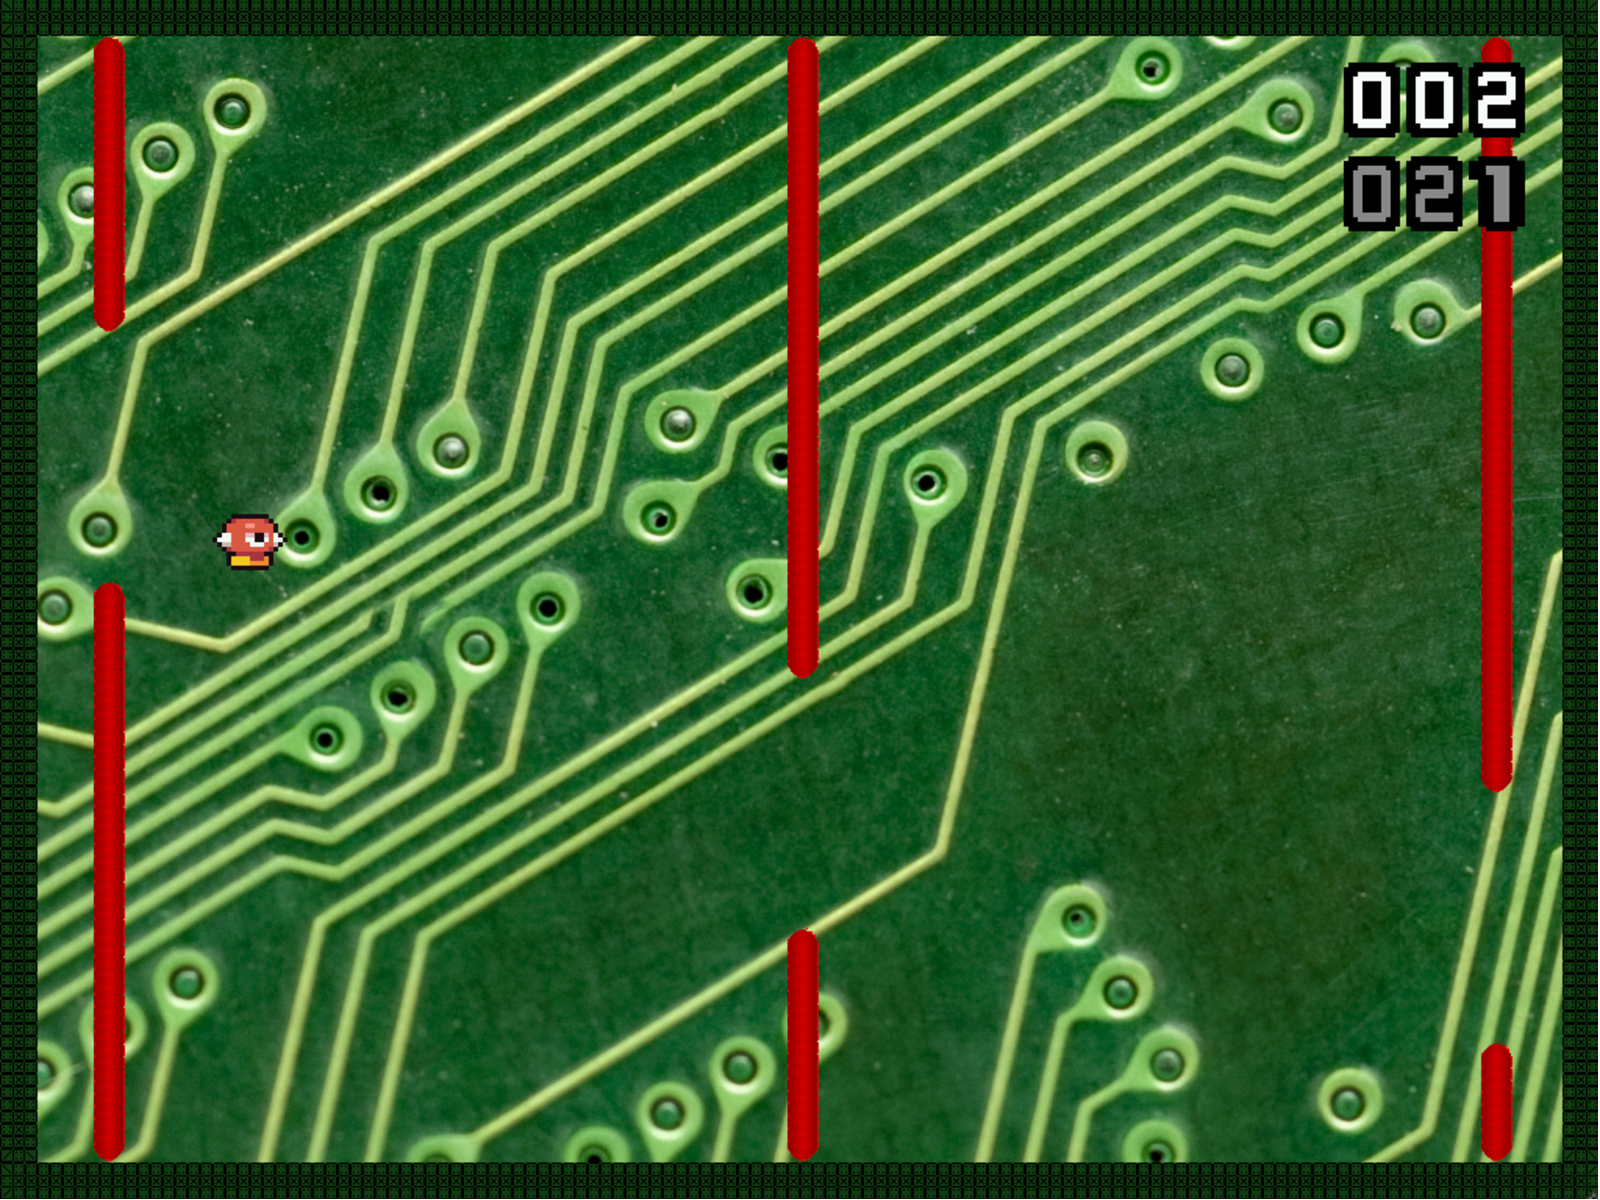
\includegraphics[width=0.6\textwidth]{arcade}
	\caption{Arcade - Singleplayer}
	\label{fig:arcade_singleplayer}
\end{figure}

\begin{figure}[H]
	\centering
	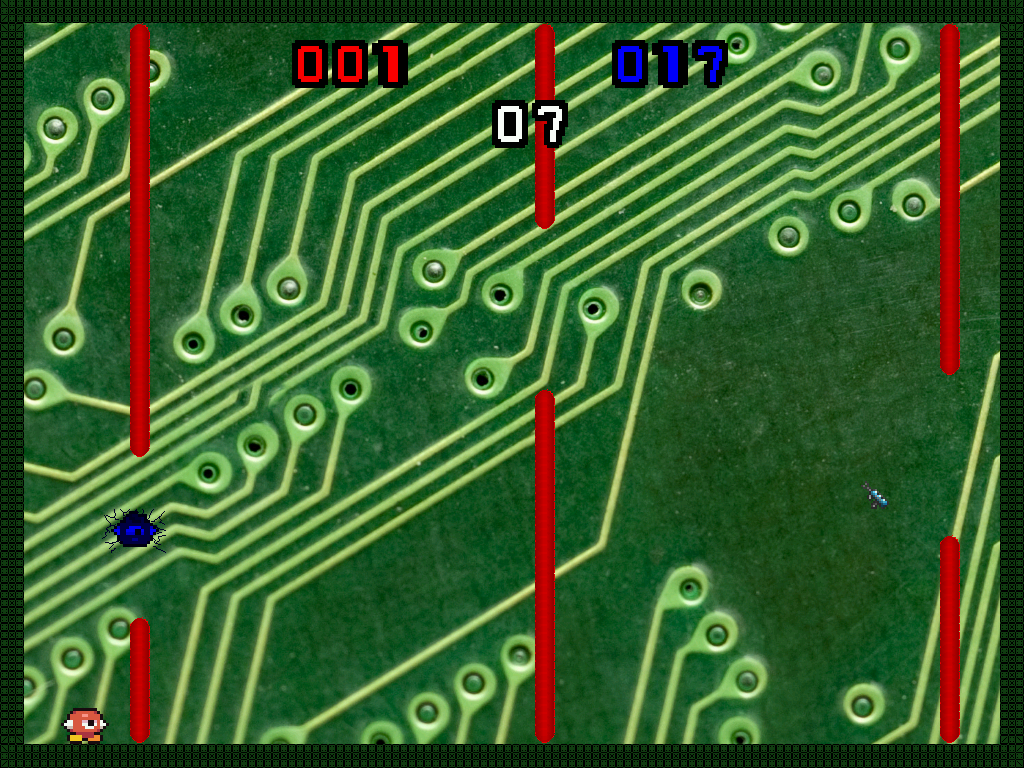
\includegraphics[width=0.6\textwidth]{arcade_versus}
	\caption{Arcade - Versus}
	\label{fig:arcade_versus}
\end{figure}


\begin{figure}[H]
	\centering
	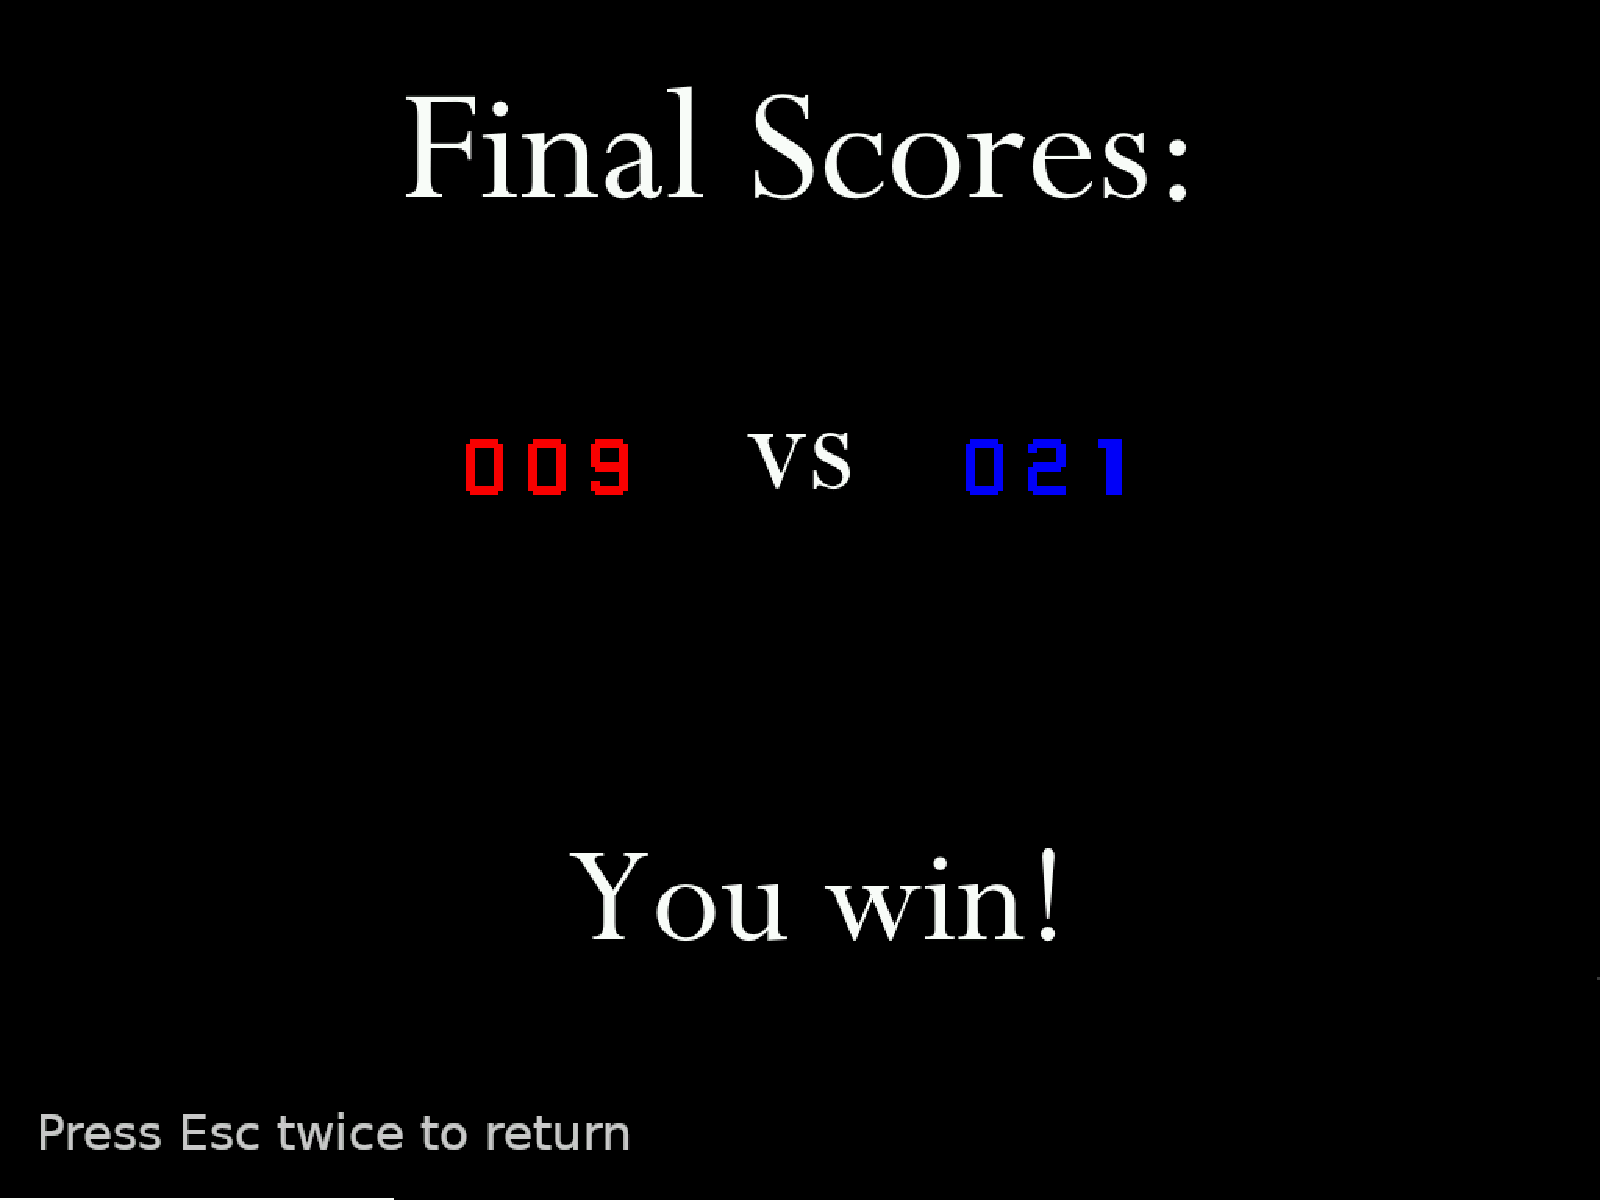
\includegraphics[width=0.6\textwidth]{arcade_you_win}
	\caption{Arcade - You Win}
	\label{fig:arcade_you_win}
\end{figure}

\section{Relatório}

Se for necessário re-compilar este relatório, em distribuições baseadas em \textit{Arch}, basta instalar a package \textit{texlive-core}, e depois correr o comando \textit{latexmk -pdf final-report.tex} a partir do diretório onde o ficheiro \textit{final-repot.tex} se encontrar.

\chapter{Estado do Projeto}

\section{Dispositivos Usados}

\begin{center}
	\begin{tabular}{|p{3cm}|p{8cm}|p{2cm}|} 
		\hline
			Dispositivo & Utilização & Interrupção \\ 
		\hline
		\hline
			Timer & Framerate handling e in-game timer  & Sim \\ 
			Teclado & Controlo da personagem 1 & Sim \\ 
			Rato & Menus e personagem 2 (switchboard) & Sim\\
			Placa Gráfica & Desenho dos menus e do jogo & Não\\
			Real Time Clock & Mini-game (switchboard, tempo demorado (campaign) e alarme para terminar o arcade mode versus & Sim\\
			Serial Port & Modos Co-Op e Versus & Sim \\
		\hline
	\end{tabular}
\end{center}

\subsection{Timer}

O timer possui como principal função atualizar o estado do jogo, assim, a cada $\frac{1}{60}$ segundos (o Timer 0 possui uma frequência de 60 Hz), todo a informação do nível (lasers ativos, coordenadas/estado do jogador, posição do rato...) é atualizada conforme os inputs do(s) utilizador(es) e o jogo é no ecrã renderizado de acordo com essa informação.
Também tem um papel importante no modo arcade ao ser utilizado para avaliar o tempo restante até o alarme do RTC terminar o jogo (foi usado o timer e o número de frames decorridos pois o RTC dava resultados diferentes nos dois PCs). Este número de frames decorrido também é responsável por ajustar a dificuldade do modo de jogo arcade.

\subsection{Teclado}

O teclado é usado para controlar a personagem 1 e o seu movimento, atraveś das teclas \textbf{W}, \textbf{A}, \textbf{S}, \textbf{D} ou pelas setas $\uparrow$, $\leftarrow$, $\downarrow$ e $\rightarrow$ e o seu salto pela tecla \textbf{Z} ou pelo \textbf{Espaço} (estas são duas das configurações de inputs mais habituais neste tipo de jogos).

Para além disso, se estiver a jogar em \textit{singleplayer}, o sentido da gravidade da personagem é trocado através da tecla \textbf{X}.

\subsection{Rato}


O rato é usado sobretudo no menu principal para selecionar o modo de jogo, clicando no botão correspondente, e no modo \textit{campaign} para controlar os \textit{sliders}, clicando e arrastando o botão esquerdo (o mesmo para a \textit{knob} no modo \textit{Co-Op}) e para selecionar o botão do \textit{laser} inativo.  
No modo de jogo \textit{co-op}, no jogador dois também é usado para impedir que uns 'balões' cheguem ao topo do ecrã e distorçam a imagem renderizada.

\subsection{Placa Gráfica}

\paragraph{}
A placa gráfica é usada para renderizar todo o jogo, por \textbf{camadas}(conforme a ordem das chamadas de render de cada elemento). É usada no modo \textbf{0x117}, que possui resolução \textbf{1024x768} e profundidade de cor \textbf{RGB 5:6:5} ($2^{16}$ cores possíveis).
Para além disso, usámos a técnica de \textbf{\textit{double buferring}} e a nossa taxa de atualização do ecrã é de \textbf{60 \textit{frames} por segundo}.

\subsection{Real Time Clock}

O \textbf{\textit{RTC}} é usado essencialmente em três vertentes diferentes: No modo \textbf{\textit{Campaign}}, com a \textbf{personagem 1}, para ler a hora de quando a personagem inicia o jogo e de quando acaba para ver quanto tempo demorou a concluir o nível; com a \textbf{personagem 2} (\textit{switchboard}) para determinar de quanto em quanto tempo surgem os \textbf{\textit{balões}} do mini-jogo, através de \textbf{\textit{alarmes}} (\textit{interrupts}); e no modo \textit{Arcade Versus} é usado um alarme para nos notificar de quando o tempo do jogo terminou.

\subsection{Serial Port}

A \textbf{\textit{serial port}} é usada para coordenadar os dois jogadores conetados nos modos \textbf{multiplayer} (Campaign - Co-Op e Arcade - Versus). No \textbf{primeiro}, as personagens 1 e 2 são controladas pelos utilizadores em máquinas separadas, sendo que estas interegam entre si do seguinte modo: A personagem 2 envia a informação no que toca aos aspetos que esta pode alterar (altura do salto, velocidade...) à personagem 1 e esta envia informação acerca do estado do jogador (powerups obtidos, morto ou vivo...). Esta informação é a mínima necessária e garante a sincronização entre os estados de ambos os ecrãs.

Já no modo \textbf{Arcade - Versus}, ambas as máquinas controlam a personagem 1 (Watt), aparecendo assim dois deles, um com a cor normal e um azul para distinguir entre os jogadores. Uma das máquinas age como \textbf{\textit{master}}, enquanto que a outra possui o papel de \textbf{\textit{slave}}. A \textbf{\textit{master}} fica encarregue de gerar a altura dos lasers aleatoriamente, com intervalos progressivamente mais curtos, alterar a velocidade dos lasers e controlar (através do alarme do RTC) quando o jogo termina para os dois jogadores. Essa informação é enviada para o \textbf{\textit{slave}}. 

Indiferente ao papel de cada máquina, ambas enviam de uma para a outra a sua posição, animação, estado (se o jogador está morto, a sua direção, se tem antigravidade ativa) e se a sua pontuação aumentou ou não.

Implementada com \textit{FIFO}s e uma receiver \textit{Queue} a nível de \textit{software}.

\chapter{Organização e Estrutura do Código}

\section{Geometry}

Peso relativo: 5\%

Módulo desenvolvido por: Tiago Silva
\newline

O módulo \textbf{\textit{Geometry}} é dividido em duas partes, \textbf{\textit{Vec2d}}, que representa um vector \textbf{bidemensional} e \textbf{\textit{Rect}}, que representa um retângulo, e serve como base do nosso sistema de coordenadas, físicas, hitboxes e colisões. É possível fazer diversas operações sobre estes dois elementos, como fazer produto escalar, soma e subtração... entre outras, no caso do Vec2d e verificar interseções, por exemplo, no caso do Rect.

\section{Bitmap} 

Peso relativo: 3\%

Módulo desenvolvido por: Eduardo Correia (40\%) e Tiago Silva (60\%)
\newline

O módulo \textbf{\textit{Bitmap}} consiste em código de nível mais baixo que carrega um \textbf{\textit{bitmap}} individual para a memória, lendo o seu header e a imagem em si --- \textit{new\_bitmap()}.
Tem a capacidade de renderizar imagens \textbf{normalmente} --- draw\_bitmap(), ou \textbf{invertidas} segundo os eixos \textit{x} --- \textit{draw\_bitmap\_reversed\_x\_axis()}, \textit{y} ---  \textit{draw\_bitmap\_reversed\_y\_axis()} ou ambos \textit{draw\_bitmap\_reversed\_both\_axis()} (garantindo a eficência).

Permite ainda renderizar o que apelidamos de um \textbf{\textit{bitmap} dinâmico}, que corresponde a representar uma imagem de tamanho indicado em \textit{runtime} (abordado no Capítulo 4).
Permite \textbf{transparência} e a aplicação de uma cor sobre o que é renderizado.
O \textit{path} absoluto para os \textit{assets} pode ser alterado como um \textit{command line argument}.
 
\section{Sprite}

Peso relativo: 5\%

Módulo desenvolvido por: Tiago Silva
\newline

O módulo \textbf{\textit{Sprite}} é, na sua essência,um \textit{wrapper} para o bitmap (tanto o normal como o dinâmico). Como acréscimo, tem uma "camada" extra que permite a animação de qualquer \textit{Sprite}, alternando o \textit{bitmap} a ser desenhada no ecrã na posição da \textit{Sprite} em questão --- \textit{set\_animation\_state()}.

\section{Game Manager}

Peso relativo: 9\%

Módulo desenvolvido por: Eduardo Correia (25\%) e Tiago Silva (75\%)
\newline

Módulo essencial que gere todos os aspetos do jogo, desde as mensagens recebidas da UART ao \textbf{driver\_receive()} e aos ciclos de \textbf{\textit{update}} e \textbf{\textit{rendering}}. É instanciado e usado como um \textit{singleton}.

\section{Hardware Manager}

Peso relativo: 1\%

Módulo desenvolvido por: Eduardo Correia (50\%) e Tiago Silva (50\%)
\newline

Este módulo foi uma tentativa de tentar encapsular ao máximo todo o conhecimento e funções responáveis por interagir com o \textbf{\textit{hardware}} num único sítio o e transparecer o mínimo possível sobre as nossas implementações internas do \textit{timer}, \textit{keyboard}, \textit{mouse}, etc..

Infelizmente existem outros módulos com um grande conhecimento destes protocolos, como o \textit{InputEvents}, o \textit{GameManager} ou tudo o que envolvesse o \textit{serial port}.

\section{Level}

Peso relativo: 8\%

Módulo desenvolvido por: Eduardo Correia (50\%) e Tiago Silva (50\%) 
\newline

Vão haver essencialmente dois níveis, um para a \textbf{Campaign} --- new\_prototype\_level() e outro para \textbf{Arcade} --- new\_arcade\_level(), sendo possível iniciar cada um destes como singleplayer ou não atraveś do parâmetro (bool is\_singleplayer).

\section{Platforms}

Peso relativo: 3\%

Módulo desenvolvido por: Tiago Silva
\newline

As plataformas agem acima de tudo como blocos construtores do nível, para definir tanto as áreas sobre as quais o jogador pode caminhar como delimitar barreiras (nomeadamente as paredes laterais para o jogador não sair fora do nível).
Possuem um SpriteDynamic para ser possível desenhá-las com uma tamanho variável e possuírmos assim maior flexibilidade no design do nível.

\section{Lasers}

Peso relativo: 5\%

Módulo desenvolvido por: Eduardo Correia (35\%) e Tiago Silva (65\%)
\newline

Os \textit{lasers} são o obstáculo mais comum que o jogador irá encontrar, tendo de evitá-los para não morrer. Cada um possui uma cor que serve também como ID para sabe que lasers estão ativos (estarão sempre todos ativos exceto o de cor correspondente ao ID inativo, controlado pelo utilizador no modo Campaign) e podem ter qualquer a dimensão desejada. 

\section{Spikes}

Peso relativo: 1\%

Módulo desenvolvido por: Eduardo Correia
\newline

São o segundo obstáculo principal do jogo. Mais simples que os lasers e ao contrário destes, são imutáveis e estáticos, não é possível "desativá-los", de modo que o jogador será de encontrar maneiras de se desviar destes para os ultrapassar. São de algum modo Platforms que o jogador não pode tocar e estão apenas presente no modo Campaign.

\section{Switchboard}

Peso relativo: 3\%

Módulo desenvolvido por: Eduardo Correia (10\%) e Tiago Silva (90\%)
\newline

Este módulo é exclusivo do modo Co-Op da Campaign e está disponível apenas para o segundo jogador. Está dotado de vários elementos UI que permitem ao segundo jogador interagir com o jogo que está a ocorrer no ecrã do primeiro jogador alterando as suas propriedades (como já foi referido anteriormente).
Possui ainda um mini-jogo em que o jogador tem de clicar em balões que surgem esporadicamente.

\section{Player}

Peso relativo: 7\%

Módulo desenvolvido por: Eduardo Correia (35\%) e Tiago Silva (65\%) 
\newline

O módulo \textit{Player} trata de gerirdor a representação de um jogador e da sua interface no nosso projeto bem como a sua interação com os restantes módulos. 

A classe \textit{PlayerTwo} apenas é utilizado no modo Arcade - Versus para representar um segundo jogador que está a jogar noutra máquina. 

\section{UI Elements}

Peso relativo: 6\%

Módulo desenvolvido por: Eduardo Correia (25\%) e Tiago Silva (75\%) 
\newline

O módulo \textit{UI Elements} consiste em vários elementos da \textit{graphical user interface} que são utilizados pelo programa. Consiste em botões, \textit{sliders}, \textit{knobs} e \textit{scoreboards}.\footnotemark

\section{Powerup}

Peso relativo: 2\%

Módulo desenvolvido por: Eduardo Correia (10\%) e Tiago Silva (90\%)
\newline

Classe que representa tanto os poderes que o \textit{Player} obtém como a saída do \textit{Level} no modo de jogo \textit{Campaign Single} e \textit{Campaign Co-op}.

\section{Timer}

Peso relativo: 4\%

Módulo desenvolvido por: Eduardo Correia (50\%) e Tiago Silva (50\%)
\newline

\textit{Código importado do Lab 2 (com melhorias)}\footnotemark[\value{footnote}]

\section{i8042}

Peso relativo: 0.5\%

Módulo desenvolvido por: Eduardo Correia (50\%) e Tiago Silva (50\%)
\newline

\textit{Código importado do Lab 2}\footnotemark

\section{Keyboard}

Peso relativo: 4\%

Módulo desenvolvido por: Eduardo Correia (50\%) e Tiago Silva (50\%)
\newline

\textit{Código importado do Lab 3}\footnotemark[\value{footnote}]

\section{Mouse}

Peso relativo: 4\%

Módulo desenvolvido por: Eduardo Correia (50\%) e Tiago Silva (50\%)
\newline

\textit{Código importado do Lab 4}\footnotemark[\value{footnote}]

\section{i8254}

Peso relativo: 0.5\%

Módulo desenvolvido por: Eduardo Correia (50\%) e Tiago Silva
\newline

\textit{Código importado do Lab 3/4}\footnotemark[\value{footnote}]

\section{Video}

Peso relativo: 6\%

Módulo desenvolvido por: Eduardo Correia (50\%) e Tiago Silva (50\%)
\newline

\textit{Código importado do Lab 5}\footnotemark[\value{footnote}]

\section{Video Macros}

Peso relativo: 1\%

Módulo desenvolvido por: Eduardo Correia (50\%) e Tiago Silva (50\%)
\newline

\textit{Código importado do Lab 5}\footnotemark[\value{footnote}]

\footnotetext{No código importado dos labs fizemos ligeiras alterações, como remover funções que não utilizamos (por exemplo, naquilo em que optássemos por usar \textit{interrupts} removemos o código que lidava com \textit{pollling}) e especificar uma abordagem geral para uma específica ao projeto, para ser mais eficaz (como usar a placa gráfica num modo apenas, correspondente ao que optámos por utilizar no nosso jogo).}

\section{RTC}

Peso relativo: 2\%

Módulo desenvolvido por: Eduardo Correia
\newline

O módulo do RTC é responsável por obter informação acerca da hora atual --- \textit{get\_date()} possuindo uma verificação antes de o fazer para obter a hora correta, bem como programar alarmes. --- \textit{rtc\_set\_alarm()}. --- rtc.c \newline

\section{UART}

Peso relativo: 5\%

Módulo desenvolvido por: Eduardo Correia (20\%) e Tiago Silva (80\%)
\newline

Este é o módulo que lida com o serial port e com a troca de informação entre os dois computadores que estarão a executar o jogo. Foi feita com FIFO's e em modo full-duplex.
 
\section{Queue}

Peso relativo: 4\%

Módulo desenvolvido por: Tiago Silva
\newline

Implementação relativamente simples da estrutura de dados \textit{queue} para uso com a UART. Foi inspirada pela implementação de um site, mas essa mesma possuía diversos erros e limitações, acabando por ser reescrita completamente na prática.

\section{InputEvents}

Peso relativo: 3\%

Módulo desenvolvido por: Eduardo Correia (40\%) e Tiago Silva (60\%)

Composto pelo \textit{KbdInputEvents} e pelo \textit{MouseInputEvents}.

Para guardar o input do \textit{keyboard} recorremos à classe \textit{KbdInputEvents}, que mantém um registo sobre todos os \textit{scancodes} de 1 \textit{byte} e sobre um subset específico de \textit{scandodes} de 2 \textit{bytes}.

Para guardar o input do rato recorremos à classe \textit{MouseInputEvents}, que expõe para o resto do programa os botões premidos pelo utilizador, se eles estão a ser premidos neste instante e se eles começaram a ser pressionados neste frame. Regista também o \textit{delta} do movimento do rato no eixo do x e y em cada frame.

\section{MouseCursor}

Peso relativo: 2\%

Módulo desenvolvido por: Tiago Silva

Representa o cursor do rato, atualizando a sua posição no ecrã e renderizando o cursor em si (quando a sua flag assim está definida).\newline

\section{Utils}

Peso relativo: 1\%

Módulo desenvolvido por: Eduardo Correia (50\%) e Tiago Silva (50\%) 
\newline

Este módulo consiste num conjunto de funções com utilidade diversa que foram usadas um pouco por todo o projeto. A maioria destas funções foram desenvolvidas ao longo dos \textit{labs} e lidam principalmente com escrita e leitura para endereços de memória, bem como manipulação de bits.

\section{MathUtils}

Peso relativo: 1\%

Módulo desenvolvido por: Eduardo Correia (50\%) e Tiago Silva (50\%)
\newline

Semelhante ao \textit{Utils}, porém, por questão de organização, decidimos separar as funcionalidades matemáticas num ficheiro à parte. A maior parte das suas funções consistem em adptações de funções já existentes (no \textit{math.h}) mas com diferentes tipos de dados (no caso caso, float, uint16\_t e uint8\_t).

\section{Main Menu}

Peso relativo: 3\%

Módulo desenvolvido por: Tiago Silva
\newline

Quando o utilizador inicia o jogo pela primeira vez ou sai de um modo jogo (Campaign ou Arcade) ele depara-se com o Main Menu. Este trata-se de um conjunto de botões que após clicadas iniciam o modo de jogo corresponde. Sempre que isso acontece, toda a informação do modo de jogo anterior (se houver algum) é libertada para prevenir memory leaks e é tratado de iniciar o próximo modo de jogo devidamente.

\section{Proj}

Peso relativo: 1\%

Módulo desenvolvido por: Tiago Silva
\newline

O módulo \textit{Proj}, por mais que possa parecer contra-intuitivo, é dos que menos tem peso no projeto, uma vez que só trata de chamar a função de iniciar o jogo --- \textit{start\_game} com o \textit{path} absoluto para as imagens passado como argumento na linha de comandos. O \textit{GameManager} trata de toda a lógica do jogo.

\section{Call Graph}

Pelo facto de utilizarmos \textit{function pointers}, não é possível gerar devidamente o gráfico do start\_game, pelo que decidimos incluir o gráfico para cada modo de jogo que temos e o menu principal.

\subsection{Menu Principal}

\begin{figure}[H]
	\centering
	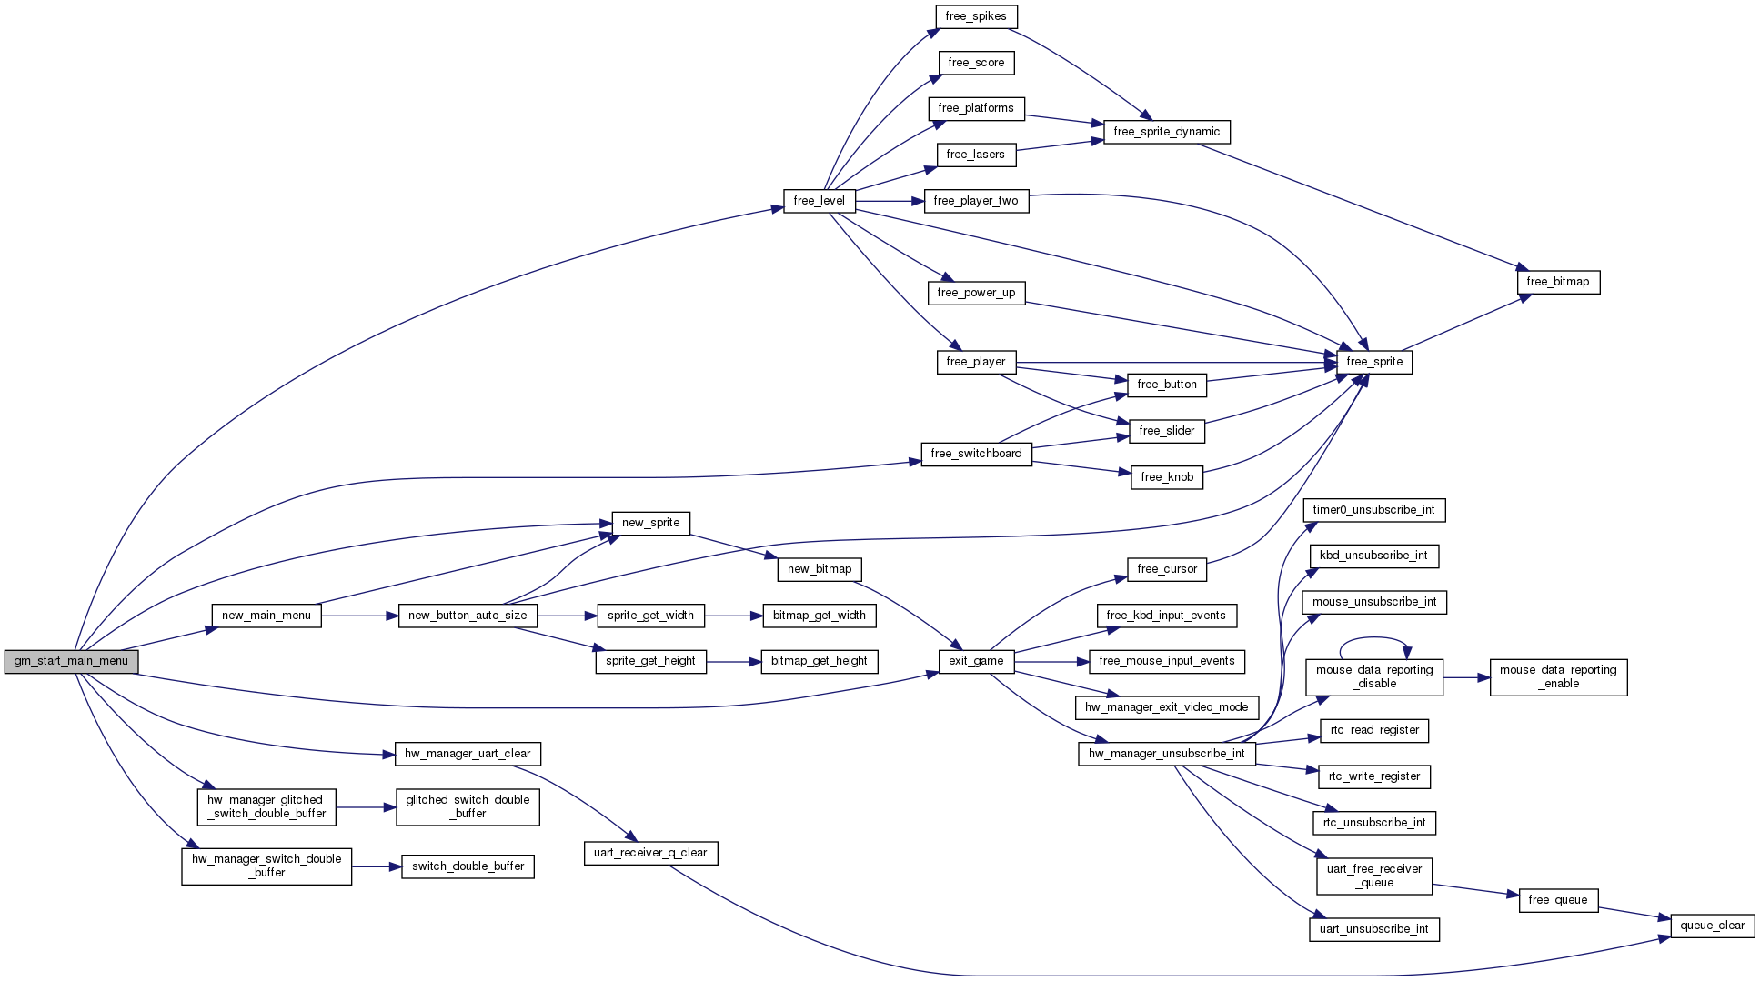
\includegraphics[width=0.9\textwidth]{gm_start_main_menu}
	\caption{Call Graph - gm\_start\_main\_menu()}
\end{figure}

\subsection{Arcade}

\begin{figure}[H]
	\centering
	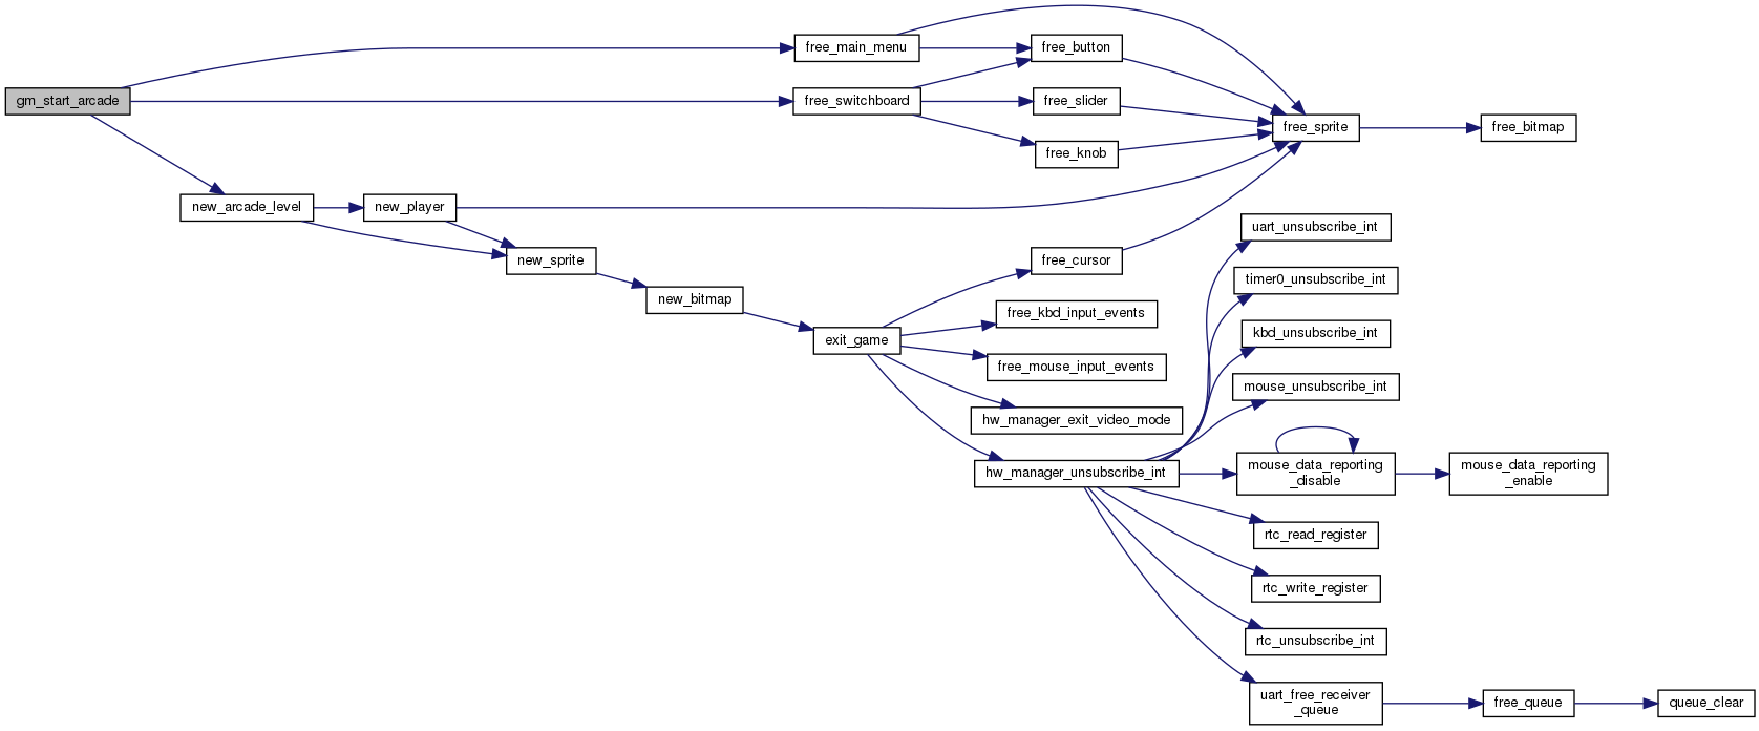
\includegraphics[width=0.9\textwidth]{gm_start_arcade}
	\caption{Call Graph - gm\_start\_arcade()}
\end{figure}

\subsection{Level}

\begin{figure}[H]
	\centering
	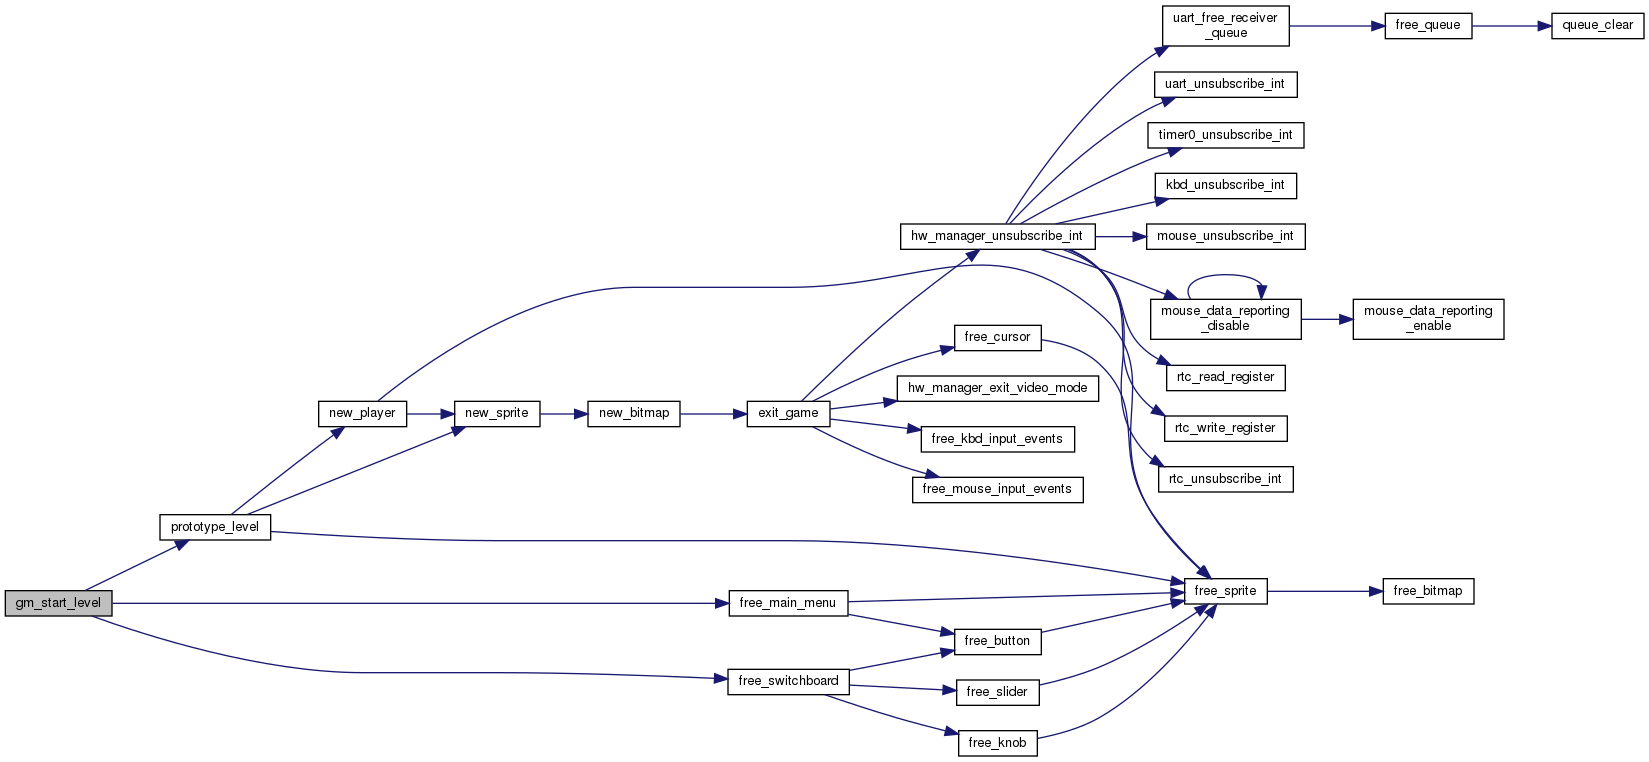
\includegraphics[width=0.9\textwidth]{gm_start_level}
	\caption{Call Graph - gm\_start\_level()}
\end{figure}

\subsection{Switchboard}

\begin{figure}[H]
	\centering
	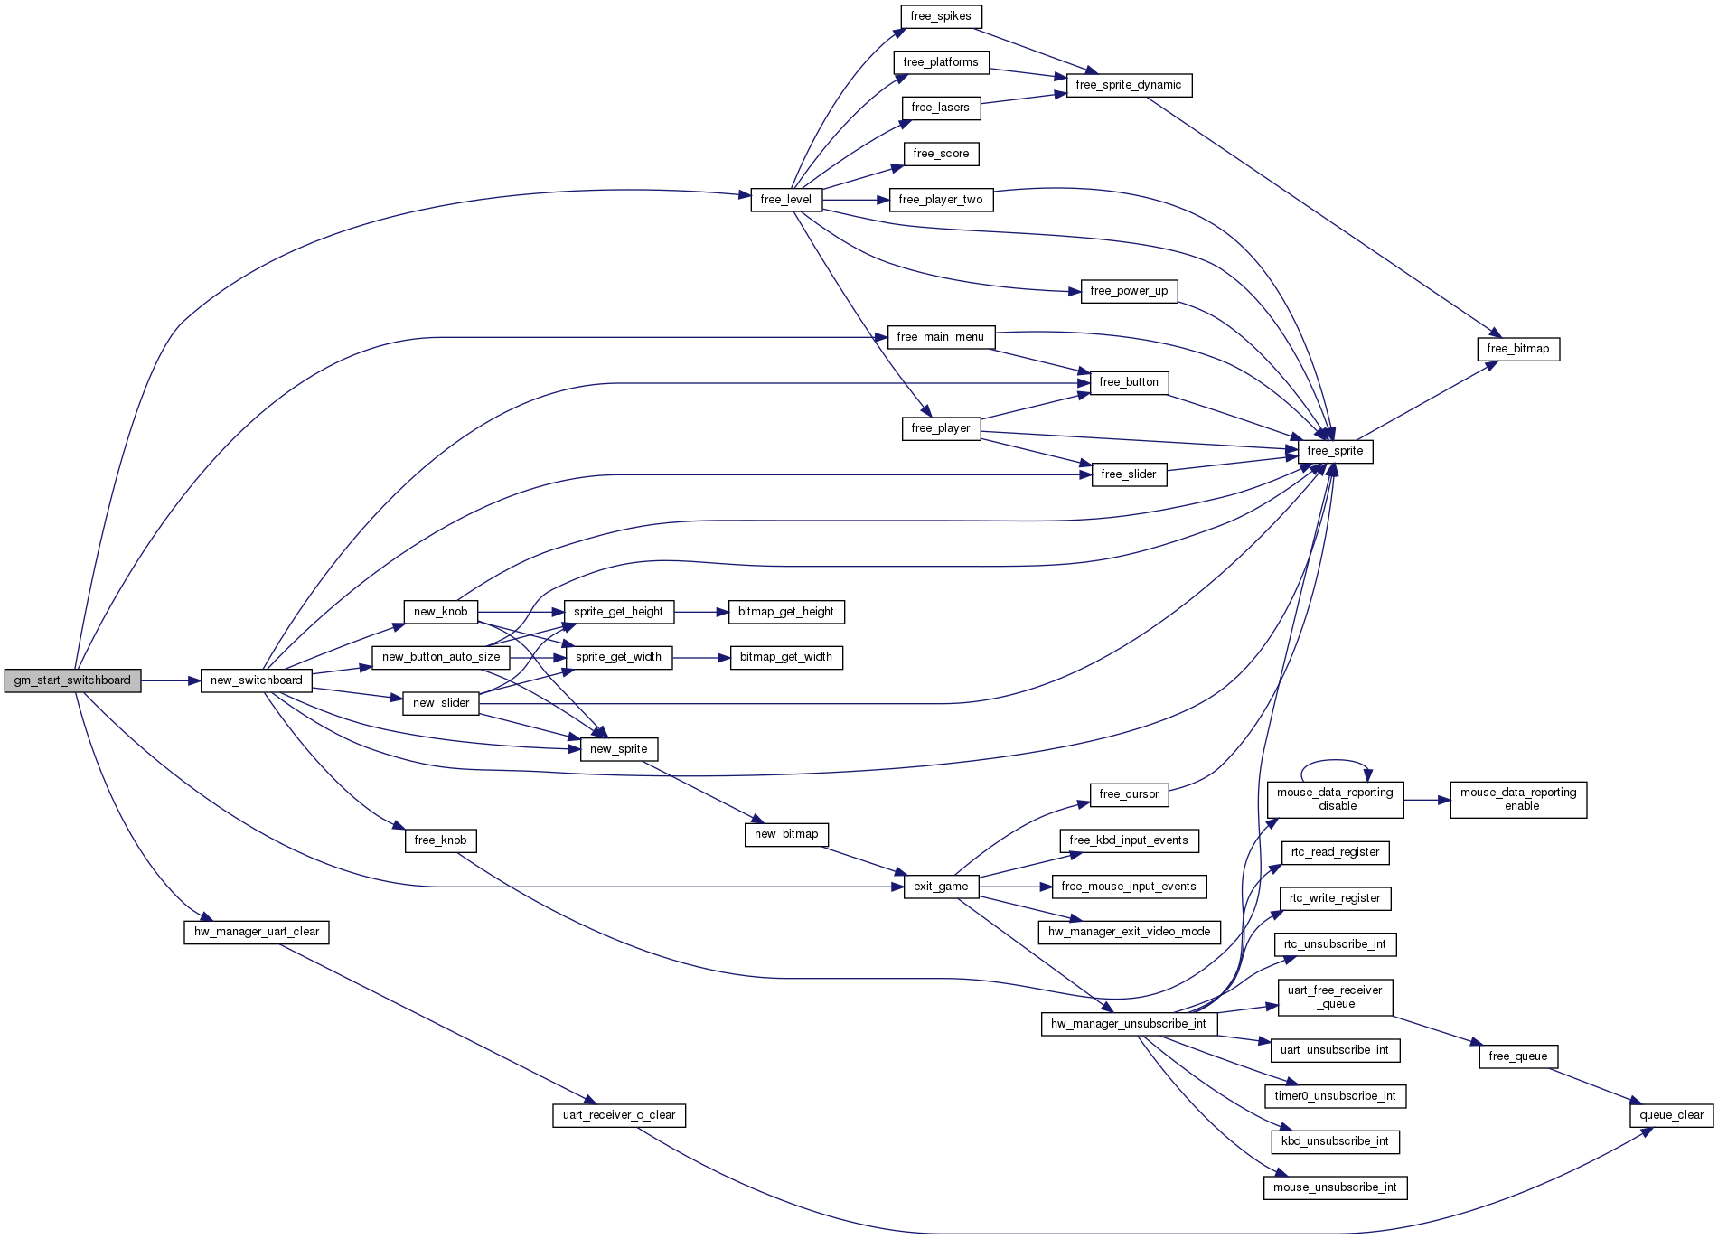
\includegraphics[width=0.9\textwidth]{gm_start_switchboard}
	\caption{Call Graph - gm\_start\_switchboard()}
\end{figure}

\section{Peso Relativo dos Módulos no Projeto}

\begin{center}
	\begin{tabular}{|c|c|} 
		\hline
			Módulo & Peso relativo (\%) \\
		\hline
		\hline
			Geometry & 5 \\
			Bitmap & 3 \\
			Sprite & 5 \\
			Game Manager & 9 \\
			Hardware Manager & 1 \\
			Level & 8 \\
			Platforms & 3 \\
			Lasers & 5 \\
			Spikes & 1 \\
			Switchboard & 3 \\ 
			Player & 7 \\
			UI Elements & 6 \\
			Powerup & 2 \\
			Timer & 4 \\
			i8042 & 0.5 \\
			Keyboard & 4 \\
			Mouse & 4 \\
			i8254 & 0.5 \\
			Video & 6 \\
			Video Macros & 1 \\
			RTC & 2 \\
			UART & 5 \\
			Queue & 4 \\
			InputEvents & 3 \\
			MouseCursor & 2 \\
			Utils & 1 \\
			Math Utils & 1 \\
			Main Menu & 3 \\
			Proj & 1 \\
		\hline
		\hline
			Total & 100 \\
		\hline
	\end{tabular}
\end{center}

\chapter{Detalhes de Implementação}

\section{Geometry}

O módulo \textit{Geometry} é dividido em duas partes, \textbf{\textit{Vec2d}} e \textbf{\textit{Rect}}, e serve como base do nosso sistema de coordenadas, físicas, hitboxes e colisões. 
\subsection{Vec2d}

Este módulo é usado para representar \textbf{vetores} de duas dimensões, e consequentemente, \textbf{pontos} no espaço (não se trata de nada mais que o vetor aplicado à origem do referencial). Cada \textbf{\textit{Vec2d}} é composto pelas suas componentes \textbf{horizontal} (\textit{x}) e \textbf{vertical} (\textit{y}), seguindo o referencial do \textit{frame buffer} (x no sentido da esquerda para a direita e y no sentido de cima para baixo).

Existe um conjunto de \textbf{operações} que podemos efetuar com esta classe, nomeadamente somar --- \textit{sum\_vec2d()}, subtrair --- \textit{subtract\_vec2d}, multiplicar por um escalar ---multiply\_by\_scalar\_vec2d()), obter a norma do vetor --- \textit{norm\_vec2d()}, o ângulo entre dois vetores (usado para a \textit{Knob}) --- \textit{angle\_vec2d()}, produto escalar --- \textit{internal\_prod\_vec2d()}, a distância entre dois pontos do plano --- \textit{distance\_vec2d()}, calcular a posição de um ponto em coordenadas polares --- \textit{circumference\_vec2d()}, entre outros (todas estas funções encontram-se expostas no \textit{Doxygen} deste módulo).

\subsection{Rect}

A classe \textit{Rect} representa, ao seu nível mais simples, \textit{retângulos}. Eles são usados para representar a \textbf{\textit{hitbox}} tanto dos diversos elementos do jogo (\textit{Player}, \textit{Lasers}, \textit{Platforms}, ...), como dos \textit{UI elements} (que área do ecrã é dedicada a ativar um botão, por exemplo).

Cada \textit{Rect} é composto pelas \textbf{coordenadas} do seu ponto superior esquerdo, tanto como pela sua \textbf{largura} e \textbf{altura}. Existem vários construtores disponíveis com propósitos diferentes: \textit{rect()}, \textit{rect\_from\_vec2d()}, \textit{rect\_from\_points()} (gera o retângulo definido por dois pontos).

\subsection{Sistema de Colisões}

O nosso sistema de colisões foi construído pensando em várias \textbf{camadas}, isto para permitir que um determinado objecto só colida com os necessários, como por exemplo, podemos querer verificar se um jogador colide com uma plataforma, ficando parado no sítio onde colidir, ou se morre por colidir com \textit{lasers} --- \textit{lasers\_collide\_player()} ou espinhos --- \textit{player\_touches\_spike()}.

\section{Rendering}

O nosso sistema de \textbf{\textit{rendering}}, tal como o nosso sistema de colisões, foi pensado como tendo várias \textbf{camadas}, isto é, sabemos que temos que desenhar o \textbf{\textit{Player}} por cima do \textbf{\textit{background}}, e que temos que desenhar os \textbf{\textit{Lasers}} por cima deles.

A solução encontrada para esta questão foi dedicar diversas funções de \textbf{\textit{rendering}} ao \textit{GameManager}. Isto permitiu-nos renderizar um nível em \textit{Campaign} --- \textit{render\_level()}, a \textit{Switchboard} --- \textit{render\_switchboard()} num dos computadores em \textit{Campaign - Co-op}, os níveis e os diversos contadores (\textit{Score}) --- \textit{render\_score()} em modo \textit{Arcade} --- \textit{render\_arcade\_single()} | \textit{render\_arcade\_versus()}, etc.. O método de trocar entre estas funções de \textit{render} será abordado quando analisarmos o \textbf{\textit{GameManager}}.

Outro aspeto peculiar é podermos aplicar \textbf{filtros} sobre o ecrã inteiro sem diminuir drasticamente a \textbf{performance}. É possível definir várias funções extra para assumirem o papel de copiar do \textbf{\textit{buffer} temporário} para o \textbf{\textit{frame buffer}}, que usam efeitos especiais, como foi realizado na \textit{Switchboard} para o efeito de o ecrã aparenter ter 'estática' na imagem (só quando o utilizador não cumpre uma tarefa corretamente) --- \textit{glitched\_switch\_double\_buffer()}. 

\subsection{Bitmap}

O código que usamos ler \textbf{bitmaps} foi parcialmente retirado da internet, mas com várias alterações para melhor se ajustar ao tipo de \textbf{\textit{bitmaps}} que usamos (criados no GIMP).

Todos os ficheiros externos necessários (\textit{.bmp}) encontram-se organizados dentro de uma pasta \textbf{\textit{assets}}, cuja localização pode ser especificada ao iniciar o jogo (até um limite de 255 carateres, incluíndo os ficheiros no interior dessa pasta).

Com o intuito de reduzir a quantidade de \textit{bitmaps} criados, ao desenhar no ecrã cada \textit{bitmap} \textbf{"normal"}, existe a opção de o desenhar alinhado à \textbf{esquerda}, ao \textbf{centro} ou à \textbf{direita} do ponto do ecrã indicado num argumento. Para além desse argumento existe ainda a possibilidade de desenhar o \textbf{simétrico} de cada \textit{bitmap} segundo quer o seu eixo (centrado no \textit{bitmap}) horizontal, vertical ou ambos. Esta segunda \textit{feature} foi especialmente útil e importante para as animações do jogador. 

Ao desenvolver o projeto considerámos necessário uma maneira de poder renderizar todas as nossas plataformas, paredes, espinhos e lasers de uma maneira mais dinâmica, para evitar criar uma nova sprite manualmente por cada objeto novo dessas classes. Assim implementamos uma função bitmap\_draw\_dynamic() que nos permite criar \textit{bitmaps} bastante reduzidos e que ocupam extremamente pouca memória RAM. Cada um destes \textit{bitmaps} pode ser subdividido em 9 quadrados, todos de tamanho igual, específico de cada imagem. A função irá depois reproduzir cada secção apropriadamente para produzir no ecrã uma imagem do tamanho pretendido.

Existe ainda a possibilidade de cada pixel ser "multiplicado" por uma cor. Devido ao custo pesado de computação desta operação, decidimos que usar uma operação bitwise entre a cor do pixel e da cor a multiplicar, visto que o efeito que ela produz seja satisfatório o suficiente para as nossas necessidades, mantendo um baixo custo computacional. Esta operação irá sempre escurecer a cor do \textit{bitmap} original, e quando aplicado a um pixel branco irá ficar apenas a cor a multiplicar. Esta propriedade foi usada a renderizar todas as plataformas e paredes. 

Todos os \textit{bitmaps} podem ser desenhados com "transparência", isto é, definimos a cor rosa, \textbf{0xFF00FF} (em RBG 888), como a cor que será sempre ignorada ao desenhar.

O path para o diretório \textit{Assets} (onde se encontram todas as imagens), pode ser alterado como um \textit{command line argument} ao correr o projeto.

\subsection{Sprite}

No nosso programa existem duas classes de \textit{sprite}: a \textbf{normal} e a \textbf{dinâmica}. A dinâmica é usada sempre que quisermos usar a função bitmap\_draw\_dynamic() referida acima, a normal é usada em todos os outros casos.

Foi tomada a decisão de implementar as animações seguindo o popular \textit{Unity}. Este \textit{game engine} tem uma propriedade \textit{Animator} que pode ser acoplado a qualquer objeto com um \textit{Renderer}. O \textit{Animator} é apenas uma máquina de estados que indica, no momento de renderizar o objeto no ecrã, qual a \textit{Sprite}, textura ou \textit{3D Model} a usar.

O sistema que decidimos implementar está imbutido diretamente na nossa classe \textit{Sprite}, que permite criar cada objeto com até 255 \textit{bitmaps}. Para permitir a instanciação de tantos \textit{bitmaps}, recorremos a um construtor que aceita um número variável de argumentos. A nossa classe tem uma propriedade "estado da animação", que indica qual dos n \textit{bitmaps} a desenhar. Este estado pode obtido e alterado através de um par de setters e getters.

A máquina de estados responsável por controlar qual o valor deste estado (por \textit{default} este valor é 0, ou seja, o primeiro \textit{bitmap}). Este tema será abordado novamente ao discutir o \textit{player}.

Cada \textit{sprite} criada também tem um \textit{offset} individual que é utilizado ao renderizar o \textit{bitmap} no ecrã. Existe ainda um getter das \textit{sprites} (\textbf{Vec2d\_t sprite\_get\_size(Sprite\_t *s)})que permite obter o tamanho do primeiro \textit{bitmap} carregado, especialmente útil para obter dinâmicamente a \textit{hitbox} do \textit{player} e dos botões.\newline

\section{User Inputs}

\subsection{KbdInputEvents}

Com o propósito de criar um \textit{dispatcher} eficiente, foi usado um \textit{map} para mapear cada \textit{scancode} ao seu valor respetivo. É registada sempre se uma tecla está a ser pressionada e se uma tecla foi pressionada durante este frame (isto é, se o utilizador empurrou para baixo a tecla).

A função \textbf{kbd\_input\_events\_process\_scancode()} trata de interpretar qualquer scancode que seja recebido do \textit{keyboard}.

Para mais permito um acesso mais simples a estas informações a partir de qualquer ponto do programa, esta classe foi tornada um \textit{singleton}, com dois getters para saber se uma tecla se encontra premida, \textbf{get\_key(KeyboardMap\_t map)}, e se uma tecla foi premida neste frame, \textbf{get\_key\_down(KeyboardMap\_t map)}.

O \textit{KeyboardMap} utilizado como argumento é um \textit{enum} com todas as teclas suportadas. Isto também permite que se o layout do teclado for diferente do \textit{default}, os scancodes podem ser alterados apenas nesse \textit{enum}.

Para detetar se uma tecla foi premida num certo frame, foi necessário limpar esse segundo map no final de cada frame, isto é, após a chamada da função \textit{update()}, para garantir que os inputs são interpretados corretamente, recorrendo à função \textbf{reset\_kbd\_input\_state()}.\newline

\subsection{MouseInputEvents e MouseCursor}

Para permitir saber se um dado botão começou a ser premido num determinado frame e para garantir que o \textit{delta} do rato entre frames é o correto, recorremos ao mesmo truque do \textit{KbdInputEvents}, utilizando a função \textbf{reset\_mouse\_input\_state()}.

\section{Graphical User Interface}

Este módulo é composto pelas classes Botão, \textit{Slider}, \textit{Knob}, \textit{Number} (usado internamente para o Score) e o \textit{Score}.

Todos os elementos de \textit{UI} com que o utilizador pode interagir (botão, \textit{sliders} e \textit{knob}) têm as propriedades de \textit{hidden} e \textit{active}. Quando a propriedade \textit{hidden} se encontra ativa, não é renderizado e não é possível o utilizador interagir com ele. Quando a propriedade \textit{active} se encontra ativa, ele é renderizado e é possível o utilizador interagir com ele (se não estiver ativo, é renderizado com uma cor mais escura e o utilizador não pode interagir com ele, propriedade usada quando um jogador não tem acesso a um \textit{power up}).

Estes possuem ainda um estado de ativo ou inativo e a qualquer momento é possível mudar o seu estado --- set\_activation(). Caso um elemento esteja inativo, a sua cor aparece ligeiramente menos saturada e não é possível interagir com o mesmo, ou seja, se for um \textit{Button}, não é clicável, se for um \textit{Slider}, não é 'arrastável' e, por último, se for uma \textit{Knob}, não é possível rodá-la. Se estiver ativo, a sua aparência é normal e já é permitida a interação com o utilizador.

Sempre que o utilizador passa o cursor por cima de algum elemento de \textit{UI} com que ele possa interagir, ele será rendered com uma saturação ligeiramente diferente, com o propósito de dar \textit{feedback} visual ao utilizador de que ele pode interagir com o elemento.

Um desafio inesperado (mas óbvio) que surgiu neste módulo foi que quando o utilizador 'agarra' num elemento de UI, por exemplo o \textit{slider} ou a \textit{knob}, temos que ter em conta o offset desde o ponto que indica onde uma \textit{Sprite} é desenhada e o ponto onde o utilizador clicou, tendo que fazer sempre um cálculo para garantir que interpretamos e renderizamos corretamente as ações do utilizador.  

\subsection{Button}

Tal como o nome indica, esta "classe" representa um simples botão com uma aparência desejada e formato retangular que pode ser clicado para ativar alguma funcionalidade.
Caso esteja ativo e o utilizador clicar nele com o cursor do rato, ativa a sua funcionalidade.

Para este propósito, cada botão pode ser instanciado com a sua pŕopria \textit{Sprite} ou usar uma já definida noutro ponto do jogo (para evitar carregar os mesmos \textit{bitmaps} em memória e duplicados.

Cada botão também tem definida uma \textit{hitbox}, isto é, a área do ecrã em que o cursor pode ativar o botão. Ao instanciar um botão temos a escolha de ajustar esta \textit{hitbox} automaticamente ao tamanho da \textit{Sprite}.

Para os botões provocarem alterações no código, cada um deles tem um apontador para função (\textbf{void (*func)()}) que é chamado quando o utilizador clica nele.

\subsection{Slider}

Uma barra vertical ou horizontal com um manípulo no seu interior que pode ser deslizado e colocado numa posição que provocará um efeito de \textit{magnitude} proporcional à posição do manípulo no \textit{Slider} relativamente à sua extremidade. Este \textit{slider} é composto por uma \textit{sprite} de \textit{background} e outra para o \textit{handle} (parte com que o utilizador interage).

Cada \textit{slider} tem um ponto inicial e final, que podem estar alinhados em qualquer direção (horizontal, vertical, diagonal), desde que o inicial seja o ponto mais acima e à esquerda. Esta restrição não traz qualquer problema, pois quando implementámos o \textit{slider} vertical para o multiplicador do salto, em que o início deveria ser em baixo, simplesmente interpretamos o input ao contrário (255 passa a 0 e vice-versa).

Tal como o botão, o slider também tem um apontador para função (\textbf{void (*func)(uint8\_t)}), que é chamada sempre que o utilizador larga a \textit{handle}, enviando como argumento uma aproximação entre [0, número de estados máximos] (normalmente 255) da posição em que o utilizador largou o \textit{handle}, desdo o ponto inicial até ao ponto final.

\subsection{Knob}

Uma espécie de 'maçaneta' que pode ser rodada, clicando na sua extremidade com o botão esquerdo do rato e arrastando-a, ativando algum efeito durante o tempo que ocorre entre o instante em que é rodada até rodar de volta à sua posição inicial.

Uma \textit{knob} tem um \textit{handle}, isto é, a componente em que o utilizador clica e arrasta pelo ecrã, um apontador para função chamado quando o utlizador larga o \textit{handle} (\textit{on\_drop}) e outro quando o \textit{handle} volta à sua posição inicial (\textit{on\_reset}).

Para resumir de forma simplificada o seu modo de funcionamento, o utilizador clica no \textit{handle} e arrasta-a na direção da posição final (mas é sempre analisado o ângulo e nunca a posição absoluta). Quando o utilizador larga o \textit{handle}, ele chama o seu apontador para função \textit{on\_drop}. O \textit{handle} irá automaticamente voltar para a sua posição original. Durante este período o utilizador não pode interagir com a \textit{Knob}. Quando o \textit{handle} volta à sua posição original, chama o seu apontador para função \textit{on\_reset} e permite novamente a interação com o utilizador.

Outra característica adicional, é que o utilizador não pode rodar na direção errada, isto é: Se a direção do início para o fim for no sentido do ponteiro do relógio, se o utilizador arrastar no sentido contrário até à posição final, o \textit{handle} não se irá mover até o utilizador voltar à posição do \textit{handle} no ecrã.

Este elemento foi bastante desafiante, visto a complexidade do método usado para determinar o ângulo e a posição do \textit{handle} dado o ângulo determinado. Foram usadas extensivamente as funções associadas ao \textit{Vec2d} de \textit{circumference\_vec2d()}, \textit{angle\_vec2d()} (que por sua vez necessita do \textit{prod\_vec\_vec2d()} e do \textit{norm\_vec2d()}), \textit{sum\_vec2d()}, \textit{subtract\_vec2d()}, entre outras.

\subsection{Number}

A classe \textbf{\textit{Number}} serve para representar um único algarismo entre 0 e 9, sendo ainda possível incrementá-lo dinamicamente por um unidade --- \textit{updade\_number()}.

\subsection{Score}

A classe \textbf{\textit{Score}} serve para representar um número com um determinado número de algarismos (\textit{Numbers}). É utilizada para mostrar a pontuação atual de um jogador no modo de jogo \textit{arcade}, o tempo restante no modo \textit{arcade versus}, e para exibir o tempo (em segundos) que o jogador demorou a concluir o nível no modo \textit{campaign} (tanto \textit{single player} como \textit{co-op}).

É possível iniciar o \textit{Score} com um valor inteiro positivo qualquer --- new\_score(), bem como repô-lo (colocar a 0) --- \textit{reset\_score()} ou mudar o seu valor --- \textit{set\_score()}. \newline

Estas duas classes, \textit{Number} e \textit{Score}, poderiam ser facilmente expandidas para renderizar texto, bastaria alterar o tipo de dados para char e renderizá-lo (a pior parte seria os \textit{Sprites} necessários para compor uma \textit{font}). Quanto à disposição do texto, bastava fazer com que o \textit{Score} deixasse de ter tamanho fixo.

\section{Level}

% -> Level editor :(
\subsection{Platforms e Spikes}

A classe Platforms representa o conjunto de plataformas que existirão em cada nível, tanto em Campaign --- \textit{prototype\_platforms()}, como em Arcade --- \textit{new\_arcade\_platforms()}. Estas podem ou não serem paredes.

Os espinhos são em tudo semelhantes às plataformas exceto pela sua aparência e pelo facto do jogador morrer ao tocar nestes. Estão apenas presentes no Level do modo Campaign.

\subsection{Lasers}

A classe Lasers representa o conjunto de lasers que existirão em cada nível. 

No modo Campaign estes serão quatro, dois azuis, um vermelho e um rosa, só duas cores de lasers é que estarão ativas de cada vez (podendo-se definir quais cores --- \textit{lasers\_set\_link\_id()}) e não mudam de posição.

Já no modo Arcade, o conjunto de lasers é todo da mesma cor (vermelho), estão sempre ativos e são gerados novos pares de lasers --- \textit{arcade\_add\_laser()}, com uma altura aleatória --- \textit{arcade\_generate\_laser\_height()} periodicamente --- \textit{arcade\_lasers\_set\_correct\_delay()}, que surgem da ponta direita do ecrã --- \textit{arcade\_spawn\_next\_laser()}, e se deslocam até à esquerda do mapa --- \textit{arcade\_move\_lasers()}, com uma certa velocidade \textit{arcade\_lasers\_set\_speed()}, sendo destruídos quando lá chegam.

A frequência a que os lasers surgem e a velocidade a que eles movem são ainda parâmetros que vão-se alterando conforme o jogador vai progredindo --- \textit{arcade\_update\_laser\_values} | \textit{arcade\_versus\_update\_laser\_values()}.

Por último, sempre que o Player toca num destes lasers, estes são repostos, tal como a sua frequência a que são gerados e a sua velocidade --- \textit{arcade\_reset\_lasers()}, caso contrário, se ele conseguir passar por entre os lasers --- \textit{arcade\_player\_passes\_lasers()} recebe um ponto.

É possível voltar atrás e passar pelo mesmo laser outra vez, mas visto a dificuldade bastante elevada desta manobra, decidimos deixá-lo no jogo, visto que se o jogador a conseguir fazer, merece o ponto extra.

\subsection{Player}

Animações

\subsection{PlayerTwo}

O PlayerTwo posui a utilidade de representar um segundo jogador que está a jogar noutro computador no modo Arcade. 

O que é um Player num PC é representado como PlayerTwo no outro.

A sua posição no ecrã e o seu estado são enviadas por UART e atualizadas no ecrã do outro jogador.

\subsection{Campaign}

% Chamar atenção de em singleplayer ter UI

\subsection{Power Ups}

Ao longo do modo Campaign, o jogador precisa de obter powerups para ganhar novas funcionalidades de modo a passar o nível. Cada vez que apanha um powerup, desbloqueia o controlo de uma mecânica adicional e só é possível obtê-los uma única vez (a não ser que o jogador morra, sendo eles repostos na sua posição inicial).

Existem portanto três powerups:
\newline

--- \textbf{Laser} - Após o jogador obter este powerup, torna possível controlar qual das três cores dos lasers está inativa, controlada pelo próprio jogador nos \textit{sliders} do canto superior esquerdo do nível, se estiver a jogar Singleplayer, e pela Switchboard se estiver a jogar Co-Op. Representada por um pequeno computador.

--- \textbf{Anti-Gravity} - Após o jogador obter este powerup, torna possível alterar o sentido da gravidade durante instantes (passando a ser puxado para o teto) através da tecla X (em Singleplayer) ou de uma \textit{Knob}  (em  modo Co-Op) que simultaneamente ilustra o tempo que o efeito de anti-gravidade estará ativo. Representada por uma maçã com um símbolo de uma seta.

--- \textbf{Exit} Ao contrário dos outros powerups, a saída não dá qualquer poder ao jogador, mas por uma questão de simplificação do código, ela está implementada como um power\_up, visto partilhar todas as características com eles (só pode ser 'apanhada' uma vez por nível, ativa uma função noutro lado para causar um efeito, tem uma Sprite). Representado como uma placa de saída de emergência fundida com o símbolo de ligação à terra.

\subsubsection{Single player}

\subsubsection{Co-op player 1 - Watt}

\subsubsection{Co-op player 2 - Switchboard}

\subsection{Arcade}

\subsubsection{Arcade Single}

\subsubsection{Arcade Versus}

\section{Game Manager}

O \textit{GameManager} é o responsável por coordenar todas as várias componentes do nosso projeto, para não mencionar o facto de o \textit{proj\_main\_loop()} estar integrado dentro da função do GameManager \textit{start\_game()}.

Esta classe é composta por apontadores para os três tipos de classes 'principais', o \textit{Level}, a \textit{Switchboard} e o \textit{MainMenu}. Tem dois \textit{arrays} de apontadores para funções que representam as diversas funções de \textit{update} e \textit{render} que existem. Um membro dado do tipo \textit{GameModeEnum} que representa o modo de jogo atual. Dois apontadores para função que representam as funções de double buffering que desenvolvemos. Diversos \textit{booleans} para sabermos os estado da UART a qualquer altura. Para finalizar, tem uma variável responsável por detetar se o utilizador premiu duas vezes a tecla Esc num curto intervalo de tempo.

\subsection{Singleton}

Como cencetualmente só pode existir um \textit{GameManager}, para permitir que o restante código seja mais simples e tenha fácil acesso ao \textit{GameManager}, decidimos torná-lo num \textbf{\textit{Singleton}}. Esta técnica muito usada na indústria dos vídeo jogos implica que só pode existir uma única instância do \textit{GameManager} na aplicação inteira. Para isto o GameManager é definido como um \textit{static GameManager *gm}, e para aceder ao GameManager fora do ficheiro game\_manager.c é utilizada a função \textit{get\_game\_manager()}, que retorna um apontador para o \textit{GameManager} e inicializa-o se ele ainda não o tiver sido.

\subsection{GameModeEnum}

Este enum representa sempre o modo de jogo atual, através da atribuição de significado a cada bit. Ou seja, sendo o BIT(0) o bit que indica se a UART é utilizada ou não, o BIT(1) a indicar se é um \textit{Level} normal (\textit{Campaign}). Assim podemos identificar unicamente o modo de jogo atual com um \textit{bitwise and}.

Mode de jogo 2 (b10) indica que nos encontramos em \textit{Campaign Singleplayer}, mas modo de jogo 3 (b11) indica que nos encontramos em \textit{Campaign Co-op Player 1}.

\subsection{Update e Render}

Devido a cada um dos modos de jogo ter um método de atualizar a informação e de a renderizar diferente, adotamos o método de ter um \textit{array} de apontadores de funções cujo índice é o próprio \textit{GameModeEnum}. Isto faz com que a chamada da função estática \textit{update()} e \textit{render()} cada uma chame dentro dela a função correta para o modo de jogo atual.

Assim evitamos a necessidade de um \textit{switch case} todos os frames para determinar qual a função correta. Para diminuir a probabilidade de \textit{segmentation faults}, as funções do array que não têm um valor possível são preenchidas com um apontador para uma função void vazia.

\subsection{Mensagens recebidas via UART}

Todas as nossas mensagens são pacotes de tamanho irregular que começam num \textit{header} predefinido e terminam num terminador \textit{Header\_Terminator}. A menor mensagem tem tamanho 2 e a maior 8. Após cada mensagem limpamos toda a \textit{Receiver Queue} até ela estar ou vazia ou encontrarmos um terminador. Propositadamente, se algum erro ocorrer na \textit{Queue}, receberemos o valor 0xFF (o valor de \textit{HEADER\_TERMINATOR}), portanto é um mecanismo de prevenção de erros. Se recebermos um \textit{header} que não estávamos à espera, essa mensagem é simplesmente eliminada.

Quando é iniciado um novo modo de jogo, a \textit{receiver Queue} do RTC é limpa, para garantir que não vamos ler mensagens antigas.

As mensagens recebidas via UART são processadas apenas pela função de \textit{update} correta, isto é, o programa ignora as mensagens de que ele não está à espera (por exemplo receber uma mensagem da \textit{Switchboard} em \textit{Arcade Mode}).
Existem duas etapas em cada função de \textit{update}: Uma primeira etapa em que os \textit{serial ports} ainda não estão 'sincronizados' (por isto entenda-se que não estão juntos no mesmo \textit{Gamemode}), depois de eles estarem 'sincronizados' ele espera um conjunto diferente de mensagens da \textit{UART}.

Em cada frame lemos e interpretamos o maior número de mensagens possíveis. Para garantir que não lemos uma mensagem incompleta no entanto, verificamos sempre se a Queue tem pelo menos o tamanho do 'pacote' que estamos a receber. Nesse caso 

\subsection{Main loop}

O \textit{main loop} está dentro da função \textit{start\_game()}. Esta última função inicializa todas as classes necessárias (\textit{InputEvents}, \textit{MouseCursor}, \textit{GameManager}), subscreve a todas as interrupções, inicializa uma seed aleatória no \textit{srand()}.

Durante o ciclo do \textit{driver\_receive()}, processamos o mais rápido possível os interrupção e aquando de uma interrupção do \textit{timer 0}, chamamos as funções \textit{update()}, \textit{render()} e a função para tratar do \textit{double buffering}, nesta ordem.

Ao terminar o \textit{start\_game()} dá \textit{unsubcribe} aos interrupts, ele liberta a memória ainda ocupada (por exemplo pelos \textit{InputEvents} ou pela \textit{Queue}) e termina o jogo.

\subsection{Outros aspetos}

A classe \textit{GameManager} também é responsável por garantir que toda a memória ocupada é libertada assim que possível, de modo a evitar memory leaks (que acreditamos ter corrigido todas) e \textit{segmentation faults}. Caso aconteça algum \textit{segmentation fault}, ao correr o programa novamente ele não irá conseguir subscrever aos interrupts, mas implementámos uma verificação nesse caso em que pede ao utilizador para correr novamente o programa (pois resolvemos o problema nesta 'iteração' do jogo).

A mecânica de premir Esc duas vezes consecutivamente para ou voltar ao \textit{MainMenu} ou sair do jogo é manuseada pelo \textit{GameManager}. Dependedo do \textit{GameModeEnum} atual ele faz a ação correta.

Seguindo a indicação do docente Souto, decidimos permitir que o \textit{path} absoluto para o diretório dos \textit{assets} seja definida como um \textit{command line argument}. Por omissão é utilizado o \textit{path} que usámos durante o desenvolvimento do programa.

\chapter{Conclusões}

Para concluir o nosso projeto, gostaríamos de realçar o que achámos de pior e melhor na cadeira de Laboratório de Computadores, constatar quais foram as nossas maiores dificuldades na elaboração do projeto final e fazer uma avaliação geral do nosso aproveitamento desta.

Em primeiro lugar, quanto aos maus aspetos desta unidade curricular gostaríamos de ressaltar o aspeto que toca à organização da informação que nos era fornecida tanto nos guiões dos \textit{Labs}, como nas transparências das aulas. 

Frequentemente tínhamos dificuldade em encontrar o que procurávamos, a documentação nem sempre estava completa e a navegação pela mesma era confusa, sugerimos portanto uma melhoria nesta vertente.

Por outro lado, a cadeira possuiu ainda um lado bastante positivo, na medida em que: Aprendemos novas abordagens e técnicas da informática, aprofundámos o nosso conhecimento de programação a baixo nível e pela primeira vez até agora no curso, tivemos um projeto de maior dimensão e também com uma maior liberdade para explorarmos ao máximo as potencialidades do que aprendemos nas aulas.

Quanto às nossas maiores dificuldades, estas foram principalmente a implementação da UART, uma vez que os Interrutps \textit{THR Empty} nem sempre funcionavam devidamente e devido ao facto do seu debug ser relativamente difícil (o que se aplica na realidade ao projeto inteiro).

Em suma, achamos que tiramos um bom proveito desta cadeira e que nos vai expandir os horizontes no futuro, gostaríamos portanto de agradecer aos docentes da cadeira pela sua prestação a leccionar, pelo esclarecimento das dúvidas que foram surgindo ao longo do semestre e pelo acompanhamento nas aulas práticas. Quanto a este último tópico, fomos constantemente coordenando com o professor os aspetos a melhorar a nível de \textit{hardware}, tendo ele salientado o facto de não enviarmos informação em quantidade e frequência o suficiente pela UART. Cremos ter corrigido essa questão com a implementação do modo Arcade - Versus e de resto, como não foram apontadas mais falhas relevantes, acreditarmos ter cumprido com as nossas expetativas para este projeto.

\paragraph{}

\end{document}